\ifx\XeTeXrevision\undefined
\pdfoutput=1 % arXiv: compile with pdfLaTeX (guarded so XeTeX-based Tectonic also works)
\fi
% When Is Cosine Similarity Enough?  --  manuscript source.
% Every number below is a macro defined in generated/numbers.tex, and every table body is a file in generated/,
% both written by src/make_tables.py from results/*.json. Figures are written by src/make_figures.py.
\documentclass[11pt]{article}
\usepackage[preprint]{acl}
\usepackage{times}
\usepackage{latexsym}
\usepackage[T1]{fontenc}
\usepackage[utf8]{inputenc}
\usepackage{microtype}
\usepackage{amsmath,amssymb}
\usepackage{booktabs}
\usepackage{graphicx}
\usepackage{makecell}
\newcommand{\yes}{\checkmark}
\newcommand{\CodeURL}{\url{https://github.com/youngaryan/cosine-vs-llm-factuality}}
% generated by src/make_tables.py -- do not edit
\newcommand{\AblFullAuc}{.817}
\newcommand{\AblFullCfAuc}{.606}
\newcommand{\AblFullFbAuc}{.637}
\newcommand{\AblFullHaluAuc}{.977}
\newcommand{\AblMinusCosineAuc}{.818}
\newcommand{\AblMinusCosineCfAuc}{.612}
\newcommand{\AblMinusCosineFbAuc}{.644}
\newcommand{\AblMinusCosineHaluAuc}{.983}
\newcommand{\AblMinusCosineLoss}{.000}
\newcommand{\AblMinusCosineLossCi}{[-.003, .002]}
\newcommand{\AblMinusEntityAuc}{.810}
\newcommand{\AblMinusEntityCfAuc}{.573}
\newcommand{\AblMinusEntityFbAuc}{.633}
\newcommand{\AblMinusEntityHaluAuc}{.974}
\newcommand{\AblMinusEntityLoss}{.008}
\newcommand{\AblMinusEntityLossCi}{[.003, .012]}
\newcommand{\AblMinusLengthAuc}{.808}
\newcommand{\AblMinusLengthCfAuc}{.607}
\newcommand{\AblMinusLengthFbAuc}{.644}
\newcommand{\AblMinusLengthHaluAuc}{.965}
\newcommand{\AblMinusLengthLoss}{.010}
\newcommand{\AblMinusLengthLossCi}{[.005, .015]}
\newcommand{\AblMinusLexicalAuc}{.794}
\newcommand{\AblMinusLexicalCfAuc}{.639}
\newcommand{\AblMinusLexicalFbAuc}{.583}
\newcommand{\AblMinusLexicalHaluAuc}{.693}
\newcommand{\AblMinusLexicalLoss}{.023}
\newcommand{\AblMinusLexicalLossCi}{[.014, .033]}
\newcommand{\AblMinusNegationAuc}{.816}
\newcommand{\AblMinusNegationCfAuc}{.608}
\newcommand{\AblMinusNegationFbAuc}{.642}
\newcommand{\AblMinusNegationHaluAuc}{.978}
\newcommand{\AblMinusNegationLoss}{.001}
\newcommand{\AblMinusNegationLossCi}{[.000, .002]}
\newcommand{\AblMinusNumberAuc}{.812}
\newcommand{\AblMinusNumberCfAuc}{.592}
\newcommand{\AblMinusNumberFbAuc}{.633}
\newcommand{\AblMinusNumberHaluAuc}{.976}
\newcommand{\AblMinusNumberLoss}{.005}
\newcommand{\AblMinusNumberLossCi}{[.002, .009]}
\newcommand{\AblOnlyCosineAuc}{.746}
\newcommand{\AblOnlyCosineCfAuc}{.580}
\newcommand{\AblOnlyCosineFbAuc}{.535}
\newcommand{\AblOnlyCosineHaluAuc}{.244}
\newcommand{\AblOnlyEntityAuc}{.663}
\newcommand{\AblOnlyEntityCfAuc}{.652}
\newcommand{\AblOnlyEntityFbAuc}{.581}
\newcommand{\AblOnlyEntityHaluAuc}{.719}
\newcommand{\AblOnlyLengthAuc}{.661}
\newcommand{\AblOnlyLengthCfAuc}{.555}
\newcommand{\AblOnlyLengthFbAuc}{.597}
\newcommand{\AblOnlyLengthHaluAuc}{.975}
\newcommand{\AblOnlyLexicalAuc}{.789}
\newcommand{\AblOnlyLexicalCfAuc}{.551}
\newcommand{\AblOnlyLexicalFbAuc}{.637}
\newcommand{\AblOnlyLexicalHaluAuc}{.973}
\newcommand{\AblOnlyNegationAuc}{.547}
\newcommand{\AblOnlyNegationCfAuc}{.563}
\newcommand{\AblOnlyNegationFbAuc}{.580}
\newcommand{\AblOnlyNegationHaluAuc}{.533}
\newcommand{\AblOnlyNumberAuc}{.565}
\newcommand{\AblOnlyNumberCfAuc}{.597}
\newcommand{\AblOnlyNumberFbAuc}{.504}
\newcommand{\AblOnlyNumberHaluAuc}{.560}
\newcommand{\CalDttBrier}{.208}
\newcommand{\CalDttEce}{.048}
\newcommand{\CalFbBrier}{.385}
\newcommand{\CalFbEce}{.417}
\newcommand{\CalHaluBrier}{.373}
\newcommand{\CalHaluEce}{.422}
\newcommand{\CalQaBrier}{.133}
\newcommand{\CalQaEce}{.117}
\newcommand{\CalSumBrier}{.176}
\newcommand{\CalSumEce}{.094}
\newcommand{\CfBertChi}{301.5}
\newcommand{\CfBertCramerV}{.22}
\newcommand{\CfBertDetect}{8.6}
\newcommand{\CfBertDetectAddition}{26.6}
\newcommand{\CfBertDetectCausal}{0.0}
\newcommand{\CfBertDetectCi}{[7.7, 9.5]}
\newcommand{\CfBertDetectDate}{2.0}
\newcommand{\CfBertDetectDirection}{1.3}
\newcommand{\CfBertDetectEntity}{6.8}
\newcommand{\CfBertDetectFar}{4.8}
\newcommand{\CfBertDetectNegation}{1.7}
\newcommand{\CfBertDetectNumber}{1.0}
\newcommand{\CfBertDetectRoleSwap}{4.0}
\newcommand{\CfBertDilFirst}{.25}
\newcommand{\CfBertDilLast}{.16}
\newcommand{\CfBertDrop}{95.9}
\newcommand{\CfBertDropAddition}{99.9}
\newcommand{\CfBertDropCausal}{83.5}
\newcommand{\CfBertDropDate}{94.8}
\newcommand{\CfBertDropDirection}{95.9}
\newcommand{\CfBertDropEntity}{98.6}
\newcommand{\CfBertDropNegation}{91.9}
\newcommand{\CfBertDropNumber}{97.2}
\newcommand{\CfBertDropRoleSwap}{93.7}
\newcommand{\CfBertFlipRej}{44.7}
\newcommand{\CfBertInv}{55.0}
\newcommand{\CfBertInvCi}{[48.8, 60.7]}
\newcommand{\CfBertOrigAcc}{63.8}
\newcommand{\CfBertOrigAccFar}{19.3}
\newcommand{\CfBertParaAcc}{58.5}
\newcommand{\CfBertParaFalseRej}{5.1}
\newcommand{\CfBertParaOrigAcc}{60.6}
\newcommand{\CfBertParaSd}{.09}
\newcommand{\CfBertSdAddition}{.70}
\newcommand{\CfBertSdCausal}{.04}
\newcommand{\CfBertSdDate}{.04}
\newcommand{\CfBertSdDirection}{.04}
\newcommand{\CfBertSdEntity}{.19}
\newcommand{\CfBertSdNegation}{.06}
\newcommand{\CfBertSdNumber}{.04}
\newcommand{\CfBertSdRoleSwap}{.12}
\newcommand{\CfBgeChi}{453.2}
\newcommand{\CfBgeCramerV}{.27}
\newcommand{\CfBgeDetect}{14.1}
\newcommand{\CfBgeDetectAddition}{35.2}
\newcommand{\CfBgeDetectCausal}{2.2}
\newcommand{\CfBgeDetectCi}{[12.9, 15.4]}
\newcommand{\CfBgeDetectDate}{2.0}
\newcommand{\CfBgeDetectDirection}{4.1}
\newcommand{\CfBgeDetectEntity}{12.9}
\newcommand{\CfBgeDetectFar}{6.2}
\newcommand{\CfBgeDetectNegation}{10.3}
\newcommand{\CfBgeDetectNumber}{2.5}
\newcommand{\CfBgeDetectRoleSwap}{1.6}
\newcommand{\CfBgeDilFirst}{.36}
\newcommand{\CfBgeDilLast}{.18}
\newcommand{\CfBgeDrop}{90.3}
\newcommand{\CfBgeDropAddition}{98.2}
\newcommand{\CfBgeDropCausal}{70.0}
\newcommand{\CfBgeDropDate}{81.1}
\newcommand{\CfBgeDropDirection}{87.1}
\newcommand{\CfBgeDropEntity}{92.7}
\newcommand{\CfBgeDropNegation}{94.3}
\newcommand{\CfBgeDropNumber}{82.3}
\newcommand{\CfBgeDropRoleSwap}{76.2}
\newcommand{\CfBgeFlipRej}{60.1}
\newcommand{\CfBgeInv}{38.2}
\newcommand{\CfBgeInvCi}{[33.0, 43.4]}
\newcommand{\CfBgeOrigAcc}{54.0}
\newcommand{\CfBgeOrigAccFar}{15.3}
\newcommand{\CfBgeParaAcc}{45.1}
\newcommand{\CfBgeParaFalseRej}{13.0}
\newcommand{\CfBgeParaOrigAcc}{51.8}
\newcommand{\CfBgeParaSd}{.08}
\newcommand{\CfBgeSdAddition}{.79}
\newcommand{\CfBgeSdCausal}{.03}
\newcommand{\CfBgeSdDate}{.05}
\newcommand{\CfBgeSdDirection}{.09}
\newcommand{\CfBgeSdEntity}{.24}
\newcommand{\CfBgeSdNegation}{.21}
\newcommand{\CfBgeSdNumber}{.04}
\newcommand{\CfBgeSdRoleSwap}{.04}
\newcommand{\CfCosChi}{590.2}
\newcommand{\CfCosCramerV}{.31}
\newcommand{\CfCosDetect}{12.0}
\newcommand{\CfCosDetectAddition}{37.0}
\newcommand{\CfCosDetectCausal}{0.7}
\newcommand{\CfCosDetectCi}{[11.0, 13.0]}
\newcommand{\CfCosDetectDate}{1.3}
\newcommand{\CfCosDetectDirection}{1.5}
\newcommand{\CfCosDetectEntity}{10.5}
\newcommand{\CfCosDetectFar}{3.8}
\newcommand{\CfCosDetectNegation}{3.2}
\newcommand{\CfCosDetectNumber}{0.4}
\newcommand{\CfCosDetectRoleSwap}{1.6}
\newcommand{\CfCosDilFirst}{.29}
\newcommand{\CfCosDilLast}{.15}
\newcommand{\CfCosDrop}{86.1}
\newcommand{\CfCosDropAddition}{98.9}
\newcommand{\CfCosDropCausal}{63.4}
\newcommand{\CfCosDropDate}{70.0}
\newcommand{\CfCosDropDirection}{79.6}
\newcommand{\CfCosDropEntity}{91.4}
\newcommand{\CfCosDropNegation}{89.9}
\newcommand{\CfCosDropNumber}{71.9}
\newcommand{\CfCosDropRoleSwap}{74.6}
\newcommand{\CfCosFlipRej}{54.1}
\newcommand{\CfCosInv}{36.6}
\newcommand{\CfCosInvCi}{[31.0, 42.3]}
\newcommand{\CfCosOrigAcc}{57.8}
\newcommand{\CfCosOrigAccFar}{10.4}
\newcommand{\CfCosParaAcc}{56.0}
\newcommand{\CfCosParaFalseRej}{1.8}
\newcommand{\CfCosParaOrigAcc}{56.5}
\newcommand{\CfCosParaSd}{.04}
\newcommand{\CfCosSdAddition}{.74}
\newcommand{\CfCosSdCausal}{.01}
\newcommand{\CfCosSdDate}{.02}
\newcommand{\CfCosSdDirection}{.04}
\newcommand{\CfCosSdEntity}{.24}
\newcommand{\CfCosSdNegation}{.09}
\newcommand{\CfCosSdNumber}{.01}
\newcommand{\CfCosSdRoleSwap}{.05}
\newcommand{\CfDilFirstBin}{4--5}
\newcommand{\CfJSmallBases}{81}
\newcommand{\CfJSmallCorrectOrder}{8.9}
\newcommand{\CfJSmallDetect}{10.7}
\newcommand{\CfJSmallDetectCi}{[4.4, 17.4]}
\newcommand{\CfJSmallFlipRej}{97.7}
\newcommand{\CfJSmallInvN}{190}
\newcommand{\CfJSmallMinusBert}{4.3}
\newcommand{\CfJSmallMinusBertCi}{[-2.7, 11.5]}
\newcommand{\CfJSmallMinusBertP}{= 0.286}
\newcommand{\CfJSmallMinusBge}{-2.3}
\newcommand{\CfJSmallMinusBgeCi}{[-10.7, 6.0]}
\newcommand{\CfJSmallMinusBgeP}{= 0.589}
\newcommand{\CfJSmallMinusCos}{2.0}
\newcommand{\CfJSmallMinusCosCi}{[-4.7, 9.2]}
\newcommand{\CfJSmallMinusCosP}{= 0.615}
\newcommand{\CfJSmallMinusNli}{-9.7}
\newcommand{\CfJSmallMinusNliCi}{[-18.3, -0.7]}
\newcommand{\CfJSmallMinusNliP}{= 0.041}
\newcommand{\CfJSmallMinusRisk}{-10.0}
\newcommand{\CfJSmallMinusRiskCi}{[-18.1, -1.9]}
\newcommand{\CfJSmallMinusRiskP}{= 0.015}
\newcommand{\CfJSmallN}{299}
\newcommand{\CfJSmallOrigAcc}{12.3}
\newcommand{\CfJSmallParaAcc}{12.3}
\newcommand{\CfJSmallParaN}{81}
\newcommand{\CfJSmallPsupInv}{9.5}
\newcommand{\CfJSmallSameBertDetect}{6.4}
\newcommand{\CfJSmallSameBgeDetect}{13.0}
\newcommand{\CfJSmallSameCosDetect}{8.7}
\newcommand{\CfJSmallSameNliDetect}{20.4}
\newcommand{\CfJSmallSameRiskDetect}{20.7}
\newcommand{\CfJSmallWrongOrder}{0.0}
\newcommand{\CfJStrongBases}{21}
\newcommand{\CfJStrongCorrectOrder}{63.8}
\newcommand{\CfJStrongDetect}{63.2}
\newcommand{\CfJStrongDetectCi}{[46.4, 78.4]}
\newcommand{\CfJStrongFlipRej}{85.5}
\newcommand{\CfJStrongInvN}{47}
\newcommand{\CfJStrongMinusBert}{60.5}
\newcommand{\CfJStrongMinusBertCi}{[43.7, 75.6]}
\newcommand{\CfJStrongMinusBertP}{< 0.0005}
\newcommand{\CfJStrongMinusBge}{47.4}
\newcommand{\CfJStrongMinusBgeCi}{[29.9, 65.2]}
\newcommand{\CfJStrongMinusBgeP}{< 0.0005}
\newcommand{\CfJStrongMinusCos}{52.6}
\newcommand{\CfJStrongMinusCosCi}{[33.8, 70.1]}
\newcommand{\CfJStrongMinusCosP}{< 0.0005}
\newcommand{\CfJStrongMinusNli}{38.2}
\newcommand{\CfJStrongMinusNliCi}{[17.1, 60.0]}
\newcommand{\CfJStrongMinusNliP}{< 0.0005}
\newcommand{\CfJStrongMinusRisk}{42.1}
\newcommand{\CfJStrongMinusRiskCi}{[23.3, 58.2]}
\newcommand{\CfJStrongMinusRiskP}{< 0.0005}
\newcommand{\CfJStrongN}{76}
\newcommand{\CfJStrongOrigAcc}{76.2}
\newcommand{\CfJStrongParaAcc}{76.2}
\newcommand{\CfJStrongParaN}{21}
\newcommand{\CfJStrongPsupInv}{10.6}
\newcommand{\CfJStrongSameBertDetect}{2.6}
\newcommand{\CfJStrongSameBgeDetect}{15.8}
\newcommand{\CfJStrongSameCosDetect}{10.5}
\newcommand{\CfJStrongSameNliDetect}{25.0}
\newcommand{\CfJStrongSameRiskDetect}{21.1}
\newcommand{\CfJStrongWrongOrder}{4.3}
\newcommand{\CfNliChi}{88.9}
\newcommand{\CfNliCramerV}{.12}
\newcommand{\CfNliDetect}{18.4}
\newcommand{\CfNliDetectAddition}{12.3}
\newcommand{\CfNliDetectCausal}{9.9}
\newcommand{\CfNliDetectCi}{[16.7, 20.1]}
\newcommand{\CfNliDetectDate}{22.4}
\newcommand{\CfNliDetectDirection}{23.6}
\newcommand{\CfNliDetectEntity}{16.0}
\newcommand{\CfNliDetectFar}{11.2}
\newcommand{\CfNliDetectNegation}{24.6}
\newcommand{\CfNliDetectNumber}{18.8}
\newcommand{\CfNliDetectRoleSwap}{19.8}
\newcommand{\CfNliDilFirst}{.59}
\newcommand{\CfNliDilLast}{.21}
\newcommand{\CfNliDrop}{88.2}
\newcommand{\CfNliDropAddition}{93.5}
\newcommand{\CfNliDropCausal}{67.0}
\newcommand{\CfNliDropDate}{90.2}
\newcommand{\CfNliDropDirection}{92.7}
\newcommand{\CfNliDropEntity}{87.8}
\newcommand{\CfNliDropNegation}{84.6}
\newcommand{\CfNliDropNumber}{87.7}
\newcommand{\CfNliDropRoleSwap}{91.3}
\newcommand{\CfNliFlipRej}{65.7}
\newcommand{\CfNliInv}{12.8}
\newcommand{\CfNliInvCi}{[9.4, 16.4]}
\newcommand{\CfNliOrigAcc}{52.3}
\newcommand{\CfNliOrigAccFar}{17.5}
\newcommand{\CfNliParaAcc}{56.5}
\newcommand{\CfNliParaFalseRej}{1.9}
\newcommand{\CfNliParaOrigAcc}{54.9}
\newcommand{\CfNliParaSd}{-.04}
\newcommand{\CfNliSdAddition}{.27}
\newcommand{\CfNliSdCausal}{.13}
\newcommand{\CfNliSdDate}{.55}
\newcommand{\CfNliSdDirection}{.56}
\newcommand{\CfNliSdEntity}{.41}
\newcommand{\CfNliSdNegation}{.59}
\newcommand{\CfNliSdNumber}{.46}
\newcommand{\CfNliSdRoleSwap}{.62}
\newcommand{\CfParaKeptPct}{80}
\newcommand{\CfRiskChi}{846.8}
\newcommand{\CfRiskChkChi}{1582.8}
\newcommand{\CfRiskChkCramerV}{.51}
\newcommand{\CfRiskChkDetect}{25.0}
\newcommand{\CfRiskChkDetectAddition}{58.2}
\newcommand{\CfRiskChkDetectCausal}{0.4}
\newcommand{\CfRiskChkDetectCi}{[23.6, 26.4]}
\newcommand{\CfRiskChkDetectDate}{10.2}
\newcommand{\CfRiskChkDetectDirection}{4.5}
\newcommand{\CfRiskChkDetectEntity}{42.9}
\newcommand{\CfRiskChkDetectFar}{9.4}
\newcommand{\CfRiskChkDetectNegation}{0.9}
\newcommand{\CfRiskChkDetectNumber}{15.7}
\newcommand{\CfRiskChkDetectRoleSwap}{4.0}
\newcommand{\CfRiskChkDilFirst}{.59}
\newcommand{\CfRiskChkDilLast}{.61}
\newcommand{\CfRiskChkDrop}{84.1}
\newcommand{\CfRiskChkDropAddition}{99.9}
\newcommand{\CfRiskChkDropCausal}{61.2}
\newcommand{\CfRiskChkDropDate}{80.6}
\newcommand{\CfRiskChkDropDirection}{80.0}
\newcommand{\CfRiskChkDropEntity}{99.2}
\newcommand{\CfRiskChkDropNegation}{55.8}
\newcommand{\CfRiskChkDropNumber}{100.0}
\newcommand{\CfRiskChkDropRoleSwap}{75.4}
\newcommand{\CfRiskChkFlipRej}{57.6}
\newcommand{\CfRiskChkInv}{36.3}
\newcommand{\CfRiskChkInvCi}{[31.6, 41.2]}
\newcommand{\CfRiskChkOrigAcc}{67.3}
\newcommand{\CfRiskChkOrigAccFar}{16.3}
\newcommand{\CfRiskChkParaAcc}{61.1}
\newcommand{\CfRiskChkParaFalseRej}{7.1}
\newcommand{\CfRiskChkParaOrigAcc}{65.8}
\newcommand{\CfRiskChkParaSd}{.07}
\newcommand{\CfRiskChkSdAddition}{1.62}
\newcommand{\CfRiskChkSdCausal}{.01}
\newcommand{\CfRiskChkSdDate}{.23}
\newcommand{\CfRiskChkSdDirection}{.10}
\newcommand{\CfRiskChkSdEntity}{.98}
\newcommand{\CfRiskChkSdNegation}{.01}
\newcommand{\CfRiskChkSdNumber}{.37}
\newcommand{\CfRiskChkSdRoleSwap}{.05}
\newcommand{\CfRiskCramerV}{.37}
\newcommand{\CfRiskDetect}{18.4}
\newcommand{\CfRiskDetectAddition}{48.3}
\newcommand{\CfRiskDetectCausal}{1.5}
\newcommand{\CfRiskDetectCi}{[17.2, 19.6]}
\newcommand{\CfRiskDetectDate}{8.5}
\newcommand{\CfRiskDetectDirection}{4.5}
\newcommand{\CfRiskDetectEntity}{19.0}
\newcommand{\CfRiskDetectFar}{10.6}
\newcommand{\CfRiskDetectNegation}{0.4}
\newcommand{\CfRiskDetectNumber}{16.6}
\newcommand{\CfRiskDetectRoleSwap}{0.0}
\newcommand{\CfRiskDilFirst}{.44}
\newcommand{\CfRiskDilLast}{.51}
\newcommand{\CfRiskDrop}{79.4}
\newcommand{\CfRiskDropAddition}{100.0}
\newcommand{\CfRiskDropCausal}{59.7}
\newcommand{\CfRiskDropDate}{95.2}
\newcommand{\CfRiskDropDirection}{99.6}
\newcommand{\CfRiskDropEntity}{98.6}
\newcommand{\CfRiskDropNegation}{25.1}
\newcommand{\CfRiskDropNumber}{100.0}
\newcommand{\CfRiskDropRoleSwap}{69.0}
\newcommand{\CfRiskFlipRej}{54.9}
\newcommand{\CfRiskInv}{50.6}
\newcommand{\CfRiskInvCi}{[46.6, 55.1]}
\newcommand{\CfRiskOrigAcc}{63.1}
\newcommand{\CfRiskOrigAccFar}{23.0}
\newcommand{\CfRiskParaAcc}{53.9}
\newcommand{\CfRiskParaFalseRej}{11.2}
\newcommand{\CfRiskParaOrigAcc}{60.1}
\newcommand{\CfRiskParaSd}{.16}
\newcommand{\CfRiskSdAddition}{1.33}
\newcommand{\CfRiskSdCausal}{.01}
\newcommand{\CfRiskSdDate}{.20}
\newcommand{\CfRiskSdDirection}{.11}
\newcommand{\CfRiskSdEntity}{.48}
\newcommand{\CfRiskSdNegation}{-.02}
\newcommand{\CfRiskSdNumber}{.46}
\newcommand{\CfRiskSdRoleSwap}{.01}
\newcommand{\CfTokPrecChi}{554.3}
\newcommand{\CfTokPrecCramerV}{.30}
\newcommand{\CfTokPrecDetect}{10.4}
\newcommand{\CfTokPrecDetectAddition}{33.9}
\newcommand{\CfTokPrecDetectCausal}{1.5}
\newcommand{\CfTokPrecDetectCi}{[9.3, 11.4]}
\newcommand{\CfTokPrecDetectDate}{1.9}
\newcommand{\CfTokPrecDetectDirection}{2.8}
\newcommand{\CfTokPrecDetectEntity}{6.6}
\newcommand{\CfTokPrecDetectFar}{7.8}
\newcommand{\CfTokPrecDetectNegation}{0.5}
\newcommand{\CfTokPrecDetectNumber}{3.1}
\newcommand{\CfTokPrecDetectRoleSwap}{0.0}
\newcommand{\CfTokPrecDilFirst}{.30}
\newcommand{\CfTokPrecDilLast}{.20}
\newcommand{\CfTokPrecDrop}{71.5}
\newcommand{\CfTokPrecDropAddition}{100.0}
\newcommand{\CfTokPrecDropCausal}{27.8}
\newcommand{\CfTokPrecDropDate}{67.8}
\newcommand{\CfTokPrecDropDirection}{97.9}
\newcommand{\CfTokPrecDropEntity}{99.9}
\newcommand{\CfTokPrecDropNegation}{14.0}
\newcommand{\CfTokPrecDropNumber}{98.8}
\newcommand{\CfTokPrecDropRoleSwap}{0.0}
\newcommand{\CfTokPrecFlipRej}{45.0}
\newcommand{\CfTokPrecInv}{75.2}
\newcommand{\CfTokPrecInvCi}{[70.3, 80.1]}
\newcommand{\CfTokPrecOrigAcc}{65.3}
\newcommand{\CfTokPrecOrigAccFar}{24.4}
\newcommand{\CfTokPrecParaAcc}{49.2}
\newcommand{\CfTokPrecParaFalseRej}{18.3}
\newcommand{\CfTokPrecParaOrigAcc}{59.6}
\newcommand{\CfTokPrecParaSd}{.20}
\newcommand{\CfTokPrecSdAddition}{.84}
\newcommand{\CfTokPrecSdCausal}{.03}
\newcommand{\CfTokPrecSdDate}{.09}
\newcommand{\CfTokPrecSdDirection}{.12}
\newcommand{\CfTokPrecSdEntity}{.22}
\newcommand{\CfTokPrecSdNegation}{.01}
\newcommand{\CfTokPrecSdNumber}{.13}
\newcommand{\CfTokPrecSdRoleSwap}{.00}
\newcommand{\CostAnsWords}{127}
\newcommand{\CostBertscoreMedian}{1,005}
\newcommand{\CostBertscoreRatio}{2.4}
\newcommand{\CostBertscoreWall}{1,039}
\newcommand{\CostBgeSmallCosineEvidenceCachedMedian}{85.1}
\newcommand{\CostBgeSmallCosineEvidenceCachedRatio}{0.2}
\newcommand{\CostBgeSmallCosineEvidenceCachedWall}{95.6}
\newcommand{\CostBgeSmallCosineMedian}{631}
\newcommand{\CostBgeSmallCosineRatio}{1.9}
\newcommand{\CostBgeSmallCosineWall}{831}
\newcommand{\CostEvWords}{376}
\newcommand{\CostJudgeSmallMedian}{10,292}
\newcommand{\CostJudgeSmallPrefixCachedMedian}{4,711}
\newcommand{\CostJudgeSmallPrefixCachedPtok}{839}
\newcommand{\CostJudgeSmallPrefixCachedRatio}{11}
\newcommand{\CostJudgeSmallPrefixCachedTokPerS}{63}
\newcommand{\CostJudgeSmallPrefixCachedWall}{4,736}
\newcommand{\CostJudgeSmallPtok}{861}
\newcommand{\CostJudgeSmallRatio}{27}
\newcommand{\CostJudgeSmallTokPerS}{70}
\newcommand{\CostJudgeSmallWall}{11,791}
\newcommand{\CostJudgeStrongMedian}{38,475}
\newcommand{\CostJudgeStrongPrefixCachedMedian}{13,547}
\newcommand{\CostJudgeStrongPrefixCachedPtok}{846}
\newcommand{\CostJudgeStrongPrefixCachedRatio}{32}
\newcommand{\CostJudgeStrongPrefixCachedTokPerS}{14}
\newcommand{\CostJudgeStrongPrefixCachedWall}{13,953}
\newcommand{\CostJudgeStrongPtok}{867}
\newcommand{\CostJudgeStrongRatio}{107}
\newcommand{\CostJudgeStrongTokPerS}{16}
\newcommand{\CostJudgeStrongWall}{46,463}
\newcommand{\CostLexicalAndChecksMedian}{1.4}
\newcommand{\CostLexicalAndChecksRatio}{0.0}
\newcommand{\CostLexicalAndChecksWall}{1.5}
\newcommand{\CostMinilmCosineEvidenceCachedMedian}{42.9}
\newcommand{\CostMinilmCosineEvidenceCachedRatio}{0.1}
\newcommand{\CostMinilmCosineEvidenceCachedWall}{49.1}
\newcommand{\CostMinilmCosineMedian}{321}
\newcommand{\CostMinilmCosineRatio}{1.0}
\newcommand{\CostMinilmCosineWall}{433}
\newcommand{\CostNliMedian}{2,302}
\newcommand{\CostNliRatio}{6.7}
\newcommand{\CostNliWall}{2,900}
\newcommand{\CostRiskFullMedian}{414}
\newcommand{\CostRiskFullRatio}{1.2}
\newcommand{\CostRiskFullWall}{513}
\newcommand{\CostSampleN}{90}
\newcommand{\CsBgeFiveCov}{25.0}
\newcommand{\CsBgeFiveCovCi}{[23.1, 27.2]}
\newcommand{\CsBgeFiveFar}{4.0}
\newcommand{\CsBgeFiveFarCi}{[2.7, 5.5]}
\newcommand{\CsBgeFiveFrr}{7.4}
\newcommand{\CsBgeTenCov}{34.2}
\newcommand{\CsBgeTenCovCi}{[32.2, 36.4]}
\newcommand{\CsBgeTenFar}{9.0}
\newcommand{\CsBgeTenFarCi}{[7.0, 11.2]}
\newcommand{\CsBgeTenFrr}{7.4}
\newcommand{\CsBgeTwentyCov}{47.1}
\newcommand{\CsBgeTwentyCovCi}{[44.9, 49.4]}
\newcommand{\CsBgeTwentyFar}{17.4}
\newcommand{\CsBgeTwentyFarCi}{[14.7, 20.3]}
\newcommand{\CsBgeTwentyFrr}{7.4}
\newcommand{\CsCosFiveCov}{20.6}
\newcommand{\CsCosFiveCovCi}{[18.9, 22.5]}
\newcommand{\CsCosFiveFar}{3.6}
\newcommand{\CsCosFiveFarCi}{[2.4, 4.9]}
\newcommand{\CsCosFiveFrr}{9.1}
\newcommand{\CsCosTenCov}{29.9}
\newcommand{\CsCosTenCovCi}{[27.9, 32.1]}
\newcommand{\CsCosTenFar}{8.0}
\newcommand{\CsCosTenFarCi}{[6.1, 10.2]}
\newcommand{\CsCosTenFrr}{9.1}
\newcommand{\CsCosTwentyCov}{43.4}
\newcommand{\CsCosTwentyCovCi}{[41.2, 45.6]}
\newcommand{\CsCosTwentyFar}{16.0}
\newcommand{\CsCosTwentyFarCi}{[13.2, 19.0]}
\newcommand{\CsCosTwentyFrr}{9.1}
\newcommand{\CsNliFiveCov}{27.4}
\newcommand{\CsNliFiveCovCi}{[25.5, 29.2]}
\newcommand{\CsNliFiveFar}{5.1}
\newcommand{\CsNliFiveFarCi}{[3.8, 6.5]}
\newcommand{\CsNliFiveFrr}{9.2}
\newcommand{\CsNliTenCov}{37.3}
\newcommand{\CsNliTenCovCi}{[35.4, 39.4]}
\newcommand{\CsNliTenFar}{11.9}
\newcommand{\CsNliTenFarCi}{[9.8, 14.0]}
\newcommand{\CsNliTenFrr}{9.2}
\newcommand{\CsNliTwentyCov}{50.7}
\newcommand{\CsNliTwentyCovCi}{[48.6, 52.7]}
\newcommand{\CsNliTwentyFar}{21.1}
\newcommand{\CsNliTwentyFarCi}{[18.1, 24.1]}
\newcommand{\CsNliTwentyFrr}{9.2}
\newcommand{\CsRiskChkFiveCov}{21.3}
\newcommand{\CsRiskChkFiveCovCi}{[19.6, 23.1]}
\newcommand{\CsRiskChkFiveFar}{4.0}
\newcommand{\CsRiskChkFiveFarCi}{[2.9, 5.2]}
\newcommand{\CsRiskChkFiveFrr}{7.7}
\newcommand{\CsRiskChkTenCov}{30.8}
\newcommand{\CsRiskChkTenCovCi}{[28.8, 32.8]}
\newcommand{\CsRiskChkTenFar}{9.8}
\newcommand{\CsRiskChkTenFarCi}{[7.8, 11.8]}
\newcommand{\CsRiskChkTenFrr}{7.7}
\newcommand{\CsRiskChkTwentyCov}{44.1}
\newcommand{\CsRiskChkTwentyCovCi}{[42.0, 46.3]}
\newcommand{\CsRiskChkTwentyFar}{19.1}
\newcommand{\CsRiskChkTwentyFarCi}{[16.4, 21.9]}
\newcommand{\CsRiskChkTwentyFrr}{7.7}
\newcommand{\CsRiskCosFiveCov}{20.1}
\newcommand{\CsRiskCosFiveCovCi}{[17.9, 22.2]}
\newcommand{\CsRiskCosFiveFar}{4.1}
\newcommand{\CsRiskCosFiveFarCi}{[2.5, 5.8]}
\newcommand{\CsRiskCosFiveFrr}{8.2}
\newcommand{\CsRiskCosTenCov}{27.2}
\newcommand{\CsRiskCosTenCovCi}{[24.9, 29.6]}
\newcommand{\CsRiskCosTenFar}{6.9}
\newcommand{\CsRiskCosTenFarCi}{[4.9, 9.1]}
\newcommand{\CsRiskCosTenFrr}{8.2}
\newcommand{\CsRiskCosTwentyCov}{40.1}
\newcommand{\CsRiskCosTwentyCovCi}{[37.7, 42.6]}
\newcommand{\CsRiskCosTwentyFar}{15.1}
\newcommand{\CsRiskCosTwentyFarCi}{[12.0, 18.4]}
\newcommand{\CsRiskCosTwentyFrr}{8.2}
\newcommand{\CsRiskFiveCov}{29.6}
\newcommand{\CsRiskFiveCovCi}{[27.4, 31.7]}
\newcommand{\CsRiskFiveFar}{5.4}
\newcommand{\CsRiskFiveFarCi}{[3.8, 7.0]}
\newcommand{\CsRiskFiveFrr}{9.4}
\newcommand{\CsRiskTenCov}{37.6}
\newcommand{\CsRiskTenCovCi}{[35.3, 39.8]}
\newcommand{\CsRiskTenFar}{8.2}
\newcommand{\CsRiskTenFarCi}{[6.4, 10.0]}
\newcommand{\CsRiskTenFrr}{9.4}
\newcommand{\CsRiskTwentyCov}{54.9}
\newcommand{\CsRiskTwentyCovCi}{[52.6, 57.2]}
\newcommand{\CsRiskTwentyFar}{20.6}
\newcommand{\CsRiskTwentyFarCi}{[17.7, 23.5]}
\newcommand{\CsRiskTwentyFrr}{9.4}
\newcommand{\CurSmallCosAurc}{.407}
\newcommand{\CurSmallCosMaxGain}{.014}
\newcommand{\CurSmallCosMeanGain}{-.003}
\newcommand{\CurSmallNliAurc}{.437}
\newcommand{\CurSmallNliMaxGain}{.024}
\newcommand{\CurSmallNliMeanGain}{.007}
\newcommand{\CurSmallRiskAurc}{.335}
\newcommand{\CurSmallRiskMaxGain}{.054}
\newcommand{\CurSmallRiskMeanGain}{.030}
\newcommand{\CurStrongCosAurc}{.382}
\newcommand{\CurStrongCosMaxGain}{.031}
\newcommand{\CurStrongCosMeanGain}{-.002}
\newcommand{\CurStrongNliAurc}{.422}
\newcommand{\CurStrongNliMaxGain}{.036}
\newcommand{\CurStrongNliMeanGain}{.001}
\newcommand{\CurStrongRiskAurc}{.392}
\newcommand{\CurStrongRiskMaxGain}{.099}
\newcommand{\CurStrongRiskMeanGain}{.028}
\newcommand{\DttBertAuc}{.617}
\newcommand{\DttBertAucCi}{[.583, .656]}
\newcommand{\DttBertBacc}{.580}
\newcommand{\DttBgeAuc}{.698}
\newcommand{\DttBgeAucCi}{[.662, .731]}
\newcommand{\DttBgeBacc}{.637}
\newcommand{\DttCosAuc}{.645}
\newcommand{\DttCosAucCi}{[.606, .683]}
\newcommand{\DttCosBacc}{.604}
\newcommand{\DttCosDocAuc}{.541}
\newcommand{\DttCosDocAucCi}{[.503, .579]}
\newcommand{\DttCosDocBacc}{.536}
\newcommand{\DttJudgeKappa}{.00}
\newcommand{\DttJudgeSmallBacc}{.502}
\newcommand{\DttJudgeSmallFar}{0.9}
\newcommand{\DttJudgeSmallFrr}{98.6}
\newcommand{\DttJudgeSmallN}{180}
\newcommand{\DttJudgeStrongBacc}{.748}
\newcommand{\DttJudgeStrongFar}{23.8}
\newcommand{\DttJudgeStrongFrr}{26.7}
\newcommand{\DttJudgeStrongN}{36}
\newcommand{\DttNliAuc}{.678}
\newcommand{\DttNliAucCi}{[.643, .713]}
\newcommand{\DttNliBacc}{.642}
\newcommand{\DttRiskAuc}{.703}
\newcommand{\DttRiskAucCi}{[.663, .743]}
\newcommand{\DttRiskBacc}{.635}
\newcommand{\DttRiskChkAuc}{.671}
\newcommand{\DttRiskChkAucCi}{[.633, .710]}
\newcommand{\DttRiskChkBacc}{.630}
\newcommand{\DttRiskCosAuc}{.615}
\newcommand{\DttRiskCosAucCi}{[.576, .655]}
\newcommand{\DttRiskCosBacc}{.585}
\newcommand{\DttStrongMinusSmall}{.248}
\newcommand{\DttStrongMinusSmallCi}{[.122, .370]}
\newcommand{\DttTokPrecAuc}{.692}
\newcommand{\DttTokPrecAucCi}{[.656, .728]}
\newcommand{\DttTokPrecBacc}{.632}
\newcommand{\ErrBaselessOnlyCos}{66.2}
\newcommand{\ErrBaselessOnlyCosFar}{4.2}
\newcommand{\ErrBaselessOnlyNli}{75.1}
\newcommand{\ErrBaselessOnlyNliFar}{3.6}
\newcommand{\ErrBaselessOnlyRisk}{67.7}
\newcommand{\ErrBaselessOnlyRiskFar}{5.1}
\newcommand{\ErrConflictOnlyCos}{62.0}
\newcommand{\ErrConflictOnlyCosFar}{3.6}
\newcommand{\ErrConflictOnlyNli}{65.9}
\newcommand{\ErrConflictOnlyNliFar}{9.8}
\newcommand{\ErrConflictOnlyRisk}{52.1}
\newcommand{\ErrConflictOnlyRiskFar}{7.5}
\newcommand{\ErrEvidentBaselessInfoCos}{69.6}
\newcommand{\ErrEvidentBaselessInfoCosFar}{3.5}
\newcommand{\ErrEvidentBaselessInfoNli}{74.9}
\newcommand{\ErrEvidentBaselessInfoNliFar}{2.2}
\newcommand{\ErrEvidentBaselessInfoRisk}{68.3}
\newcommand{\ErrEvidentBaselessInfoRiskFar}{4.2}
\newcommand{\ErrEvidentConflictCos}{67.3}
\newcommand{\ErrEvidentConflictCosFar}{3.1}
\newcommand{\ErrEvidentConflictNli}{69.7}
\newcommand{\ErrEvidentConflictNliFar}{6.5}
\newcommand{\ErrEvidentConflictRisk}{57.7}
\newcommand{\ErrEvidentConflictRiskFar}{5.9}
\newcommand{\ErrSubtleBaselessInfoCos}{68.1}
\newcommand{\ErrSubtleBaselessInfoCosFar}{4.3}
\newcommand{\ErrSubtleBaselessInfoNli}{77.3}
\newcommand{\ErrSubtleBaselessInfoNliFar}{4.3}
\newcommand{\ErrSubtleBaselessInfoRisk}{71.6}
\newcommand{\ErrSubtleBaselessInfoRiskFar}{5.7}
\newcommand{\ErrSubtleConflictCos}{73.3}
\newcommand{\ErrSubtleConflictCosFar}{0.0}
\newcommand{\ErrSubtleConflictNli}{73.3}
\newcommand{\ErrSubtleConflictNliFar}{6.7}
\newcommand{\ErrSubtleConflictRisk}{66.7}
\newcommand{\ErrSubtleConflictRiskFar}{0.0}
\newcommand{\ErrSubtleOnlyCos}{58.4}
\newcommand{\ErrSubtleOnlyCosFar}{3.9}
\newcommand{\ErrSubtleOnlyNli}{74.0}
\newcommand{\ErrSubtleOnlyNliFar}{7.8}
\newcommand{\ErrSubtleOnlyRisk}{64.9}
\newcommand{\ErrSubtleOnlyRiskFar}{6.5}
\newcommand{\EvBertAuc}{.737}
\newcommand{\EvBertBacc}{.687}
\newcommand{\EvBertFar}{29.9}
\newcommand{\EvContainAuc}{.880}
\newcommand{\EvContainBacc}{.880}
\newcommand{\EvContainFar}{3.4}
\newcommand{\EvContainMinusSmall}{.068}
\newcommand{\EvContainMinusSmallCi}{[.030, .111]}
\newcommand{\EvContainMinusStrong}{.022}
\newcommand{\EvContainMinusStrongCi}{[-.036, .087]}
\newcommand{\EvContainSubSmallBacc}{.884}
\newcommand{\EvContainSubStrongBacc}{.903}
\newcommand{\EvCosAuc}{.802}
\newcommand{\EvCosBacc}{.738}
\newcommand{\EvCosFar}{27.9}
\newcommand{\EvCosMinusSmall}{-.074}
\newcommand{\EvCosMinusSmallCi}{[-.121, -.026]}
\newcommand{\EvCosMinusStrong}{-.139}
\newcommand{\EvCosMinusStrongCi}{[-.237, -.044]}
\newcommand{\EvCosSubSmallBacc}{.742}
\newcommand{\EvCosSubStrongBacc}{.742}
\newcommand{\EvCsCosCov}{42.3}
\newcommand{\EvCsCosEsc}{57.8}
\newcommand{\EvCsCosFar}{6.2}
\newcommand{\EvCsCosFrr}{8.9}
\newcommand{\EvCsCosSysBacc}{.824}
\newcommand{\EvCsRiskCov}{94.0}
\newcommand{\EvCsRiskEsc}{4.5}
\newcommand{\EvCsRiskFar}{5.3}
\newcommand{\EvCsRiskFrr}{9.0}
\newcommand{\EvCsRiskSysBacc}{.925}
\newcommand{\EvCsTokfCov}{58.4}
\newcommand{\EvCsTokfEsc}{38.0}
\newcommand{\EvCsTokfFar}{6.2}
\newcommand{\EvCsTokfFrr}{8.8}
\newcommand{\EvCsTokfSysBacc}{.858}
\newcommand{\EvEmAuc}{.582}
\newcommand{\EvEmBacc}{.582}
\newcommand{\EvEmFar}{0.2}
\newcommand{\EvJudgeKappa}{.61}
\newcommand{\EvJudgeSmallBacc}{.815}
\newcommand{\EvJudgeSmallBaccCi}{[.777, .849]}
\newcommand{\EvJudgeSmallN}{600}
\newcommand{\EvJudgeStrongBacc}{.881}
\newcommand{\EvJudgeStrongBaccCi}{[.827, .924]}
\newcommand{\EvJudgeStrongN}{150}
\newcommand{\EvNliAuc}{.884}
\newcommand{\EvNliBacc}{.820}
\newcommand{\EvNliFar}{24.1}
\newcommand{\EvRiskAuc}{.957}
\newcommand{\EvRiskBacc}{.901}
\newcommand{\EvRiskFar}{11.0}
\newcommand{\EvRiskMinusSmall}{.102}
\newcommand{\EvRiskMinusSmallCi}{[.064, .143]}
\newcommand{\EvRiskMinusStrong}{.065}
\newcommand{\EvRiskMinusStrongCi}{[.025, .110]}
\newcommand{\EvRiskSubSmallBacc}{.917}
\newcommand{\EvRiskSubStrongBacc}{.947}
\newcommand{\EvStrongMinusSmall}{.071}
\newcommand{\EvStrongMinusSmallCi}{[-.009, .160]}
\newcommand{\EvTokfAuc}{.874}
\newcommand{\EvTokfBacc}{.811}
\newcommand{\EvTokfFar}{32.4}
\newcommand{\FbBertAuc}{.569}
\newcommand{\FbBertAucCi}{[.499, .639]}
\newcommand{\FbBertBacc}{.525}
\newcommand{\FbBestCosAuc}{.412}
\newcommand{\FbBestJudgeSmallBacc}{.535}
\newcommand{\FbBestNliAuc}{.460}
\newcommand{\FbBestRiskAuc}{.466}
\newcommand{\FbBgeAuc}{.522}
\newcommand{\FbBgeAucCi}{[.465, .577]}
\newcommand{\FbBgeBacc}{.498}
\newcommand{\FbCosAuc}{.513}
\newcommand{\FbCosAucCi}{[.453, .573]}
\newcommand{\FbCosBacc}{.513}
\newcommand{\FbCosDocAuc}{.576}
\newcommand{\FbCosDocAucCi}{[.491, .658]}
\newcommand{\FbCosDocBacc}{.536}
\newcommand{\FbInCosCov}{21.2}
\newcommand{\FbInCosFar}{10.8}
\newcommand{\FbInCosFrr}{10.8}
\newcommand{\FbInRiskCov}{27.6}
\newcommand{\FbInRiskFar}{7.9}
\newcommand{\FbInRiskFrr}{8.2}
\newcommand{\FbJudgeKappa}{.04}
\newcommand{\FbJudgeSmallBacc}{.528}
\newcommand{\FbJudgeSmallFar}{14.6}
\newcommand{\FbJudgeSmallFrr}{79.7}
\newcommand{\FbJudgeSmallN}{500}
\newcommand{\FbJudgeStrongBacc}{.533}
\newcommand{\FbJudgeStrongFar}{90.6}
\newcommand{\FbJudgeStrongFrr}{2.8}
\newcommand{\FbJudgeStrongN}{100}
\newcommand{\FbNliAuc}{.546}
\newcommand{\FbNliAucCi}{[.460, .627]}
\newcommand{\FbNliBacc}{.544}
\newcommand{\FbOodCosCov}{33.4}
\newcommand{\FbOodCosFar}{14.9}
\newcommand{\FbOodCosFrr}{20.9}
\newcommand{\FbOodRiskCov}{37.4}
\newcommand{\FbOodRiskFar}{22.8}
\newcommand{\FbOodRiskFrr}{5.1}
\newcommand{\FbRiskAuc}{.637}
\newcommand{\FbRiskAucCi}{[.554, .718]}
\newcommand{\FbRiskBacc}{.595}
\newcommand{\FbRiskChkAuc}{.572}
\newcommand{\FbRiskChkAucCi}{[.494, .649]}
\newcommand{\FbRiskChkBacc}{.574}
\newcommand{\FbRiskCosAuc}{.535}
\newcommand{\FbRiskCosAucCi}{[.470, .598]}
\newcommand{\FbRiskCosBacc}{.520}
\newcommand{\FbStrongMinusSmall}{-.069}
\newcommand{\FbStrongMinusSmallCi}{[-.200, .080]}
\newcommand{\FbTokPrecAuc}{.619}
\newcommand{\FbTokPrecAucCi}{[.535, .706]}
\newcommand{\FbTokPrecBacc}{.592}
\newcommand{\GbmDttAuc}{.732}
\newcommand{\GbmFbAuc}{.626}
\newcommand{\GbmHaluAuc}{.910}
\newcommand{\GbmQaAuc}{.784}
\newcommand{\GbmSumAuc}{.670}
\newcommand{\HaluBertAuc}{.329}
\newcommand{\HaluBertAucCi}{[.308, .352]}
\newcommand{\HaluBertBacc}{.499}
\newcommand{\HaluBgeAuc}{.247}
\newcommand{\HaluBgeAucCi}{[.226, .267]}
\newcommand{\HaluBgeBacc}{.500}
\newcommand{\HaluCosAuc}{.251}
\newcommand{\HaluCosAucCi}{[.231, .272]}
\newcommand{\HaluCosBacc}{.498}
\newcommand{\HaluCosDocAuc}{.237}
\newcommand{\HaluCosDocAucCi}{[.217, .257]}
\newcommand{\HaluCosDocBacc}{.500}
\newcommand{\HaluNliAuc}{.747}
\newcommand{\HaluNliAucCi}{[.725, .770]}
\newcommand{\HaluNliBacc}{.748}
\newcommand{\HaluRiskAuc}{.977}
\newcommand{\HaluRiskAucCi}{[.970, .983]}
\newcommand{\HaluRiskBacc}{.954}
\newcommand{\HaluRiskChkAuc}{.304}
\newcommand{\HaluRiskChkAucCi}{[.282, .327]}
\newcommand{\HaluRiskChkBacc}{.499}
\newcommand{\HaluRiskCosAuc}{.244}
\newcommand{\HaluRiskCosAucCi}{[.223, .264]}
\newcommand{\HaluRiskCosBacc}{.498}
\newcommand{\HaluTokPrecAuc}{.898}
\newcommand{\HaluTokPrecAucCi}{[.882, .912]}
\newcommand{\HaluTokPrecBacc}{.916}
\newcommand{\HfourBgeDiff}{4.4}
\newcommand{\HfourBgeDiffCi}{[2.7, 6.1]}
\newcommand{\HfourBgeP}{< 0.0005}
\newcommand{\HfourHolm}{\le 0.002}
\newcommand{\HfourNliDiff}{6.7}
\newcommand{\HfourNliDiffCi}{[4.3, 9.1]}
\newcommand{\HfourNliP}{< 0.0005}
\newcommand{\HfourRaw}{\le 0.001}
\newcommand{\HfourRiskChkDiff}{0.7}
\newcommand{\HfourRiskChkDiffCi}{[-1.6, 3.0]}
\newcommand{\HfourRiskChkP}{= 0.564}
\newcommand{\HfourRiskDiff}{9.0}
\newcommand{\HfourRiskDiffCi}{[6.4, 11.5]}
\newcommand{\HfourRiskP}{< 0.0005}
\newcommand{\HfourSysDiff}{.069}
\newcommand{\HfourSysDiffCi}{[.039, .101]}
\newcommand{\HoneJudgeHolm}{= 0.615}
\newcommand{\HoneJudgeMinusCos}{2.0}
\newcommand{\HoneJudgeMinusCosCi}{[-4.7, 9.2]}
\newcommand{\HoneJudgeRaw}{= 0.615}
\newcommand{\HoneNliHolm}{\le 0.002}
\newcommand{\HoneNliMinusCos}{6.4}
\newcommand{\HoneNliMinusCosCi}{[4.6, 8.2]}
\newcommand{\HoneNliRaw}{\le 0.001}
\newcommand{\HthreeCells}{20}
\newcommand{\HthreeExceed}{7}
\newcommand{\HthreeHolm}{= 0.020}
\newcommand{\HthreePBonf}{0.010}
\newcommand{\HthreeRaw}{= 0.010}
\newcommand{\HtwoBertPerm}{< 0.0005}
\newcommand{\HtwoBertRejHi}{62.2}
\newcommand{\HtwoBertRejLo}{33.7}
\newcommand{\HtwoBgePerm}{< 0.0005}
\newcommand{\HtwoBgeRejHi}{81.6}
\newcommand{\HtwoBgeRejLo}{41.8}
\newcommand{\HtwoCosPerm}{< 0.0005}
\newcommand{\HtwoCosRejHi}{79.2}
\newcommand{\HtwoCosRejLo}{34.1}
\newcommand{\HtwoNliPerm}{< 0.0005}
\newcommand{\HtwoNliRejHi}{83.3}
\newcommand{\HtwoNliRejLo}{50.2}
\newcommand{\HtwoRiskPerm}{< 0.0005}
\newcommand{\HtwoRiskRejHi}{84.2}
\newcommand{\HtwoRiskRejLo}{35.0}
\newcommand{\HwCores}{12}
\newcommand{\HwCpu}{AMD64 Family 25 Model 116 Stepping 1, AuthenticAMD}
\newcommand{\HwRam}{30.7}
\newcommand{\HwThreads}{6}
\newcommand{\JudgeSmallCalls}{1,635}
\newcommand{\JudgeSmallFailures}{0}
\newcommand{\JudgeSmallInsufPct}{0.2}
\newcommand{\JudgeSmallModel}{llama3.2:3b}
\newcommand{\JudgeStrongCalls}{358}
\newcommand{\JudgeStrongFailures}{0}
\newcommand{\JudgeStrongInsufPct}{6.7}
\newcommand{\JudgeStrongModel}{qwen2.5:14b}
\newcommand{\LrDttAuc}{.703}
\newcommand{\LrFbAuc}{.637}
\newcommand{\LrHaluAuc}{.977}
\newcommand{\LrQaAuc}{.808}
\newcommand{\LrSumAuc}{.673}
\newcommand{\NBoot}{2,000}
\newcommand{\NCfAddition}{1,517}
\newcommand{\NCfBases}{1,517}
\newcommand{\NCfCausal}{273}
\newcommand{\NCfDate}{540}
\newcommand{\NCfDirection}{466}
\newcommand{\NCfEntity}{1,018}
\newcommand{\NCfInv}{476}
\newcommand{\NCfMatched}{3,804}
\newcommand{\NCfNegation}{1,432}
\newcommand{\NCfNumber}{773}
\newcommand{\NCfPairs}{6,145}
\newcommand{\NCfPara}{193}
\newcommand{\NCfParaAttempted}{240}
\newcommand{\NCfRoleSwap}{126}
\newcommand{\NExclImproper}{590}
\newcommand{\NExclRefusal}{144}
\newcommand{\NExclTrunc}{29}
\newcommand{\NTestEvouna}{7,096}
\newcommand{\NTestFaith}{5,175}
\newcommand{\NTestNatural}{12,271}
\newcommand{\NTestRagtruth}{2,675}
\newcommand{\PoolBertAuc}{.756}
\newcommand{\PoolBertBacc}{.568}
\newcommand{\PoolBertBaccCi}{[.547, .590]}
\newcommand{\PoolBertFar}{50.7}
\newcommand{\PoolBgeAuc}{.757}
\newcommand{\PoolBgeBacc}{.591}
\newcommand{\PoolBgeBaccCi}{[.572, .611]}
\newcommand{\PoolBgeFar}{33.8}
\newcommand{\PoolCosAuc}{.703}
\newcommand{\PoolCosBacc}{.611}
\newcommand{\PoolCosBaccCi}{[.592, .630]}
\newcommand{\PoolCosDocAuc}{.722}
\newcommand{\PoolCosDocBacc}{.551}
\newcommand{\PoolCosDocBaccCi}{[.526, .577]}
\newcommand{\PoolCosDocFar}{40.3}
\newcommand{\PoolCosFar}{33.2}
\newcommand{\PoolNliAuc}{.744}
\newcommand{\PoolNliBacc}{.613}
\newcommand{\PoolNliBaccCi}{[.594, .633]}
\newcommand{\PoolNliFar}{27.7}
\newcommand{\PoolRiskAuc}{.817}
\newcommand{\PoolRiskBacc}{.631}
\newcommand{\PoolRiskBaccCi}{[.609, .652]}
\newcommand{\PoolRiskChkAuc}{.773}
\newcommand{\PoolRiskChkBacc}{.673}
\newcommand{\PoolRiskChkBaccCi}{[.654, .691]}
\newcommand{\PoolRiskChkFar}{29.6}
\newcommand{\PoolRiskCosAuc}{.746}
\newcommand{\PoolRiskCosBacc}{.575}
\newcommand{\PoolRiskCosBaccCi}{[.553, .597]}
\newcommand{\PoolRiskCosFar}{36.2}
\newcommand{\PoolRiskFar}{37.2}
\newcommand{\PoolTokPrecAuc}{.791}
\newcommand{\PoolTokPrecBacc}{.586}
\newcommand{\PoolTokPrecBaccCi}{[.564, .607]}
\newcommand{\PoolTokPrecFar}{45.6}
\newcommand{\QaBertAuc}{.723}
\newcommand{\QaBertAucCi}{[.675, .768]}
\newcommand{\QaBertBacc}{.649}
\newcommand{\QaBgeAuc}{.689}
\newcommand{\QaBgeAucCi}{[.639, .737]}
\newcommand{\QaBgeBacc}{.643}
\newcommand{\QaCosAuc}{.683}
\newcommand{\QaCosAucCi}{[.633, .730]}
\newcommand{\QaCosBacc}{.626}
\newcommand{\QaCosDocAuc}{.523}
\newcommand{\QaCosDocAucCi}{[.470, .570]}
\newcommand{\QaCosDocBacc}{.521}
\newcommand{\QaJudgeKappa}{.29}
\newcommand{\QaJudgeSmallBacc}{.576}
\newcommand{\QaJudgeSmallFar}{0.0}
\newcommand{\QaJudgeSmallFrr}{84.8}
\newcommand{\QaJudgeSmallN}{175}
\newcommand{\QaJudgeStrongBacc}{.815}
\newcommand{\QaJudgeStrongFar}{11.1}
\newcommand{\QaJudgeStrongFrr}{25.9}
\newcommand{\QaJudgeStrongN}{36}
\newcommand{\QaNliAuc}{.654}
\newcommand{\QaNliAucCi}{[.606, .702]}
\newcommand{\QaNliBacc}{.630}
\newcommand{\QaRiskAuc}{.808}
\newcommand{\QaRiskAucCi}{[.764, .846]}
\newcommand{\QaRiskBacc}{.739}
\newcommand{\QaRiskChkAuc}{.721}
\newcommand{\QaRiskChkAucCi}{[.667, .772]}
\newcommand{\QaRiskChkBacc}{.661}
\newcommand{\QaRiskCosAuc}{.666}
\newcommand{\QaRiskCosAucCi}{[.617, .713]}
\newcommand{\QaRiskCosBacc}{.628}
\newcommand{\QaStrongMinusSmall}{.185}
\newcommand{\QaStrongMinusSmallCi}{[-.010, .292]}
\newcommand{\QaTokPrecAuc}{.723}
\newcommand{\QaTokPrecAucCi}{[.674, .765]}
\newcommand{\QaTokPrecBacc}{.640}
\newcommand{\Seed}{20261116}
\newcommand{\SensAgree}{74.9}
\newcommand{\SensBaccOne}{.550}
\newcommand{\SensBaccTwo}{.581}
\newcommand{\SensFarOne}{0.0}
\newcommand{\SensFarTwo}{16.7}
\newcommand{\SensFrrOne}{89.9}
\newcommand{\SensFrrTwo}{67.2}
\newcommand{\SensKappa}{.17}
\newcommand{\SensN}{179}
\newcommand{\ShGenCosOpenWeightToOpenWeight}{3.6}
\newcommand{\ShGenCosOpenWeightToOpenai}{3.4}
\newcommand{\ShGenCosOpenaiToOpenWeight}{1.6}
\newcommand{\ShGenCosOpenaiToOpenai}{1.1}
\newcommand{\ShGenNliOpenWeightToOpenWeight}{5.0}
\newcommand{\ShGenNliOpenWeightToOpenai}{5.7}
\newcommand{\ShGenNliOpenaiToOpenWeight}{0.8}
\newcommand{\ShGenNliOpenaiToOpenai}{1.1}
\newcommand{\ShGenRiskOpenWeightToOpenWeight}{4.2}
\newcommand{\ShGenRiskOpenWeightToOpenai}{4.5}
\newcommand{\ShGenRiskOpenaiToOpenWeight}{1.1}
\newcommand{\ShGenRiskOpenaiToOpenai}{0.0}
\newcommand{\ShLenCosLongToLong}{4.9}
\newcommand{\ShLenCosLongToShort}{12.4}
\newcommand{\ShLenCosShortToLong}{0.9}
\newcommand{\ShLenCosShortToShort}{2.5}
\newcommand{\ShLenNliLongToLong}{5.8}
\newcommand{\ShLenNliLongToShort}{17.1}
\newcommand{\ShLenNliShortToLong}{1.0}
\newcommand{\ShLenNliShortToShort}{3.4}
\newcommand{\ShLenRiskLongToLong}{4.6}
\newcommand{\ShLenRiskLongToShort}{23.0}
\newcommand{\ShLenRiskShortToLong}{0.7}
\newcommand{\ShLenRiskShortToShort}{3.4}
\newcommand{\SumBertAuc}{.619}
\newcommand{\SumBertAucCi}{[.579, .661]}
\newcommand{\SumBertBacc}{.585}
\newcommand{\SumBgeAuc}{.648}
\newcommand{\SumBgeAucCi}{[.605, .689]}
\newcommand{\SumBgeBacc}{.614}
\newcommand{\SumCosAuc}{.620}
\newcommand{\SumCosAucCi}{[.578, .663]}
\newcommand{\SumCosBacc}{.597}
\newcommand{\SumCosDocAuc}{.593}
\newcommand{\SumCosDocAucCi}{[.551, .635]}
\newcommand{\SumCosDocBacc}{.540}
\newcommand{\SumJudgeKappa}{.01}
\newcommand{\SumJudgeSmallBacc}{.578}
\newcommand{\SumJudgeSmallFar}{5.4}
\newcommand{\SumJudgeSmallFrr}{79.0}
\newcommand{\SumJudgeSmallN}{180}
\newcommand{\SumJudgeStrongBacc}{.667}
\newcommand{\SumJudgeStrongFar}{66.7}
\newcommand{\SumJudgeStrongFrr}{0.0}
\newcommand{\SumJudgeStrongN}{36}
\newcommand{\SumNliAuc}{.678}
\newcommand{\SumNliAucCi}{[.639, .716]}
\newcommand{\SumNliBacc}{.599}
\newcommand{\SumRiskAuc}{.673}
\newcommand{\SumRiskAucCi}{[.636, .713]}
\newcommand{\SumRiskBacc}{.612}
\newcommand{\SumRiskChkAuc}{.626}
\newcommand{\SumRiskChkAucCi}{[.587, .668]}
\newcommand{\SumRiskChkBacc}{.589}
\newcommand{\SumRiskCosAuc}{.622}
\newcommand{\SumRiskCosAucCi}{[.580, .662]}
\newcommand{\SumRiskCosBacc}{.585}
\newcommand{\SumStrongMinusSmall}{.130}
\newcommand{\SumStrongMinusSmallCi}{[-.008, .259]}
\newcommand{\SumTokPrecAuc}{.676}
\newcommand{\SumTokPrecAucCi}{[.636, .715]}
\newcommand{\SumTokPrecBacc}{.616}
\newcommand{\SysSmallCosFiveBacc}{.581}
\newcommand{\SysSmallCosFiveBaccCi}{[.550, .613]}
\newcommand{\SysSmallCosFiveDiff}{.015}
\newcommand{\SysSmallCosFiveDiffCi}{[-.009, .041]}
\newcommand{\SysSmallCosFiveEsc}{75.9}
\newcommand{\SysSmallCosFiveFar}{7.1}
\newcommand{\SysSmallCosFiveFarCi}{[3.3, 11.4]}
\newcommand{\SysSmallCosFiveJudgeSec}{5868}
\newcommand{\SysSmallCosFiveRand}{.579}
\newcommand{\SysSmallCosFiveSaved}{24.1}
\newcommand{\SysSmallCosTenBacc}{.594}
\newcommand{\SysSmallCosTenBaccCi}{[.559, .627]}
\newcommand{\SysSmallCosTenDiff}{.028}
\newcommand{\SysSmallCosTenDiffCi}{[-.004, .060]}
\newcommand{\SysSmallCosTenEsc}{67.1}
\newcommand{\SysSmallCosTenFar}{13.1}
\newcommand{\SysSmallCosTenFarCi}{[7.6, 19.6]}
\newcommand{\SysSmallCosTenJudgeSec}{5190}
\newcommand{\SysSmallCosTenRand}{.587}
\newcommand{\SysSmallCosTenSaved}{32.9}
\newcommand{\SysSmallCosTwentyBacc}{.625}
\newcommand{\SysSmallCosTwentyBaccCi}{[.585, .663]}
\newcommand{\SysSmallCosTwentyDiff}{.059}
\newcommand{\SysSmallCosTwentyDiffCi}{[.020, .096]}
\newcommand{\SysSmallCosTwentyEsc}{53.8}
\newcommand{\SysSmallCosTwentyFar}{20.2}
\newcommand{\SysSmallCosTwentyFarCi}{[13.4, 27.5]}
\newcommand{\SysSmallCosTwentyJudgeSec}{4155}
\newcommand{\SysSmallCosTwentyRand}{.593}
\newcommand{\SysSmallCosTwentySaved}{46.2}
\newcommand{\SysSmallJudgeBacc}{.566}
\newcommand{\SysSmallJudgeBaccCi}{[.543, .592]}
\newcommand{\SysSmallJudgeFar}{1.6}
\newcommand{\SysSmallJudgeFrr}{85.2}
\newcommand{\SysSmallN}{535}
\newcommand{\SysSmallNeverBertBacc}{.567}
\newcommand{\SysSmallNeverBertDiff}{.001}
\newcommand{\SysSmallNeverBertDiffCi}{[-.055, .056]}
\newcommand{\SysSmallNeverBgeBacc}{.559}
\newcommand{\SysSmallNeverBgeDiff}{-.006}
\newcommand{\SysSmallNeverBgeDiffCi}{[-.057, .041]}
\newcommand{\SysSmallNeverCosBacc}{.625}
\newcommand{\SysSmallNeverCosDiff}{.059}
\newcommand{\SysSmallNeverCosDiffCi}{[.015, .100]}
\newcommand{\SysSmallNeverNliBacc}{.585}
\newcommand{\SysSmallNeverNliDiff}{.019}
\newcommand{\SysSmallNeverNliDiffCi}{[-.030, .068]}
\newcommand{\SysSmallNeverRiskBacc}{.634}
\newcommand{\SysSmallNeverRiskDiff}{.068}
\newcommand{\SysSmallNeverRiskDiffCi}{[.017, .117]}
\newcommand{\SysSmallNeverTokPrecBacc}{.569}
\newcommand{\SysSmallNeverTokPrecDiff}{.004}
\newcommand{\SysSmallNeverTokPrecDiffCi}{[-.051, .063]}
\newcommand{\SysSmallNliFiveBacc}{.583}
\newcommand{\SysSmallNliFiveBaccCi}{[.551, .616]}
\newcommand{\SysSmallNliFiveDiff}{.017}
\newcommand{\SysSmallNliFiveDiffCi}{[-.009, .045]}
\newcommand{\SysSmallNliFiveEsc}{73.3}
\newcommand{\SysSmallNliFiveFar}{10.9}
\newcommand{\SysSmallNliFiveFarCi}{[6.3, 15.8]}
\newcommand{\SysSmallNliFiveJudgeSec}{5673}
\newcommand{\SysSmallNliFiveRand}{.571}
\newcommand{\SysSmallNliFiveSaved}{26.7}
\newcommand{\SysSmallNliTenBacc}{.608}
\newcommand{\SysSmallNliTenBaccCi}{[.573, .643]}
\newcommand{\SysSmallNliTenDiff}{.043}
\newcommand{\SysSmallNliTenDiffCi}{[.013, .072]}
\newcommand{\SysSmallNliTenEsc}{63.4}
\newcommand{\SysSmallNliTenFar}{16.4}
\newcommand{\SysSmallNliTenFarCi}{[11.4, 21.8]}
\newcommand{\SysSmallNliTenJudgeSec}{4867}
\newcommand{\SysSmallNliTenRand}{.572}
\newcommand{\SysSmallNliTenSaved}{36.6}
\newcommand{\SysSmallNliTwentyBacc}{.619}
\newcommand{\SysSmallNliTwentyBaccCi}{[.577, .659]}
\newcommand{\SysSmallNliTwentyDiff}{.053}
\newcommand{\SysSmallNliTwentyDiffCi}{[.014, .093]}
\newcommand{\SysSmallNliTwentyEsc}{49.2}
\newcommand{\SysSmallNliTwentyFar}{27.3}
\newcommand{\SysSmallNliTwentyFarCi}{[21.5, 33.8]}
\newcommand{\SysSmallNliTwentyJudgeSec}{3831}
\newcommand{\SysSmallNliTwentyRand}{.576}
\newcommand{\SysSmallNliTwentySaved}{50.8}
\newcommand{\SysSmallRiskChkFiveBacc}{.595}
\newcommand{\SysSmallRiskChkFiveBaccCi}{[.566, .625]}
\newcommand{\SysSmallRiskChkFiveDiff}{.029}
\newcommand{\SysSmallRiskChkFiveDiffCi}{[.007, .051]}
\newcommand{\SysSmallRiskChkFiveEsc}{77.9}
\newcommand{\SysSmallRiskChkFiveFar}{4.4}
\newcommand{\SysSmallRiskChkFiveFarCi}{[1.6, 7.5]}
\newcommand{\SysSmallRiskChkFiveJudgeSec}{5919}
\newcommand{\SysSmallRiskChkFiveRand}{.596}
\newcommand{\SysSmallRiskChkFiveSaved}{22.1}
\newcommand{\SysSmallRiskChkTenBacc}{.631}
\newcommand{\SysSmallRiskChkTenBaccCi}{[.599, .665]}
\newcommand{\SysSmallRiskChkTenDiff}{.065}
\newcommand{\SysSmallRiskChkTenDiffCi}{[.036, .094]}
\newcommand{\SysSmallRiskChkTenEsc}{67.9}
\newcommand{\SysSmallRiskChkTenFar}{8.7}
\newcommand{\SysSmallRiskChkTenFarCi}{[5.1, 12.9]}
\newcommand{\SysSmallRiskChkTenJudgeSec}{5088}
\newcommand{\SysSmallRiskChkTenRand}{.610}
\newcommand{\SysSmallRiskChkTenSaved}{32.1}
\newcommand{\SysSmallRiskChkTwentyBacc}{.643}
\newcommand{\SysSmallRiskChkTwentyBaccCi}{[.605, .681]}
\newcommand{\SysSmallRiskChkTwentyDiff}{.077}
\newcommand{\SysSmallRiskChkTwentyDiffCi}{[.040, .113]}
\newcommand{\SysSmallRiskChkTwentyEsc}{53.1}
\newcommand{\SysSmallRiskChkTwentyFar}{19.1}
\newcommand{\SysSmallRiskChkTwentyFarCi}{[13.2, 25.1]}
\newcommand{\SysSmallRiskChkTwentyJudgeSec}{3894}
\newcommand{\SysSmallRiskChkTwentyRand}{.631}
\newcommand{\SysSmallRiskChkTwentySaved}{46.9}
\newcommand{\SysSmallRiskFiveBacc}{.635}
\newcommand{\SysSmallRiskFiveBaccCi}{[.601, .671]}
\newcommand{\SysSmallRiskFiveDiff}{.069}
\newcommand{\SysSmallRiskFiveDiffCi}{[.039, .101]}
\newcommand{\SysSmallRiskFiveEsc}{64.5}
\newcommand{\SysSmallRiskFiveFar}{7.7}
\newcommand{\SysSmallRiskFiveFarCi}{[4.2, 12.0]}
\newcommand{\SysSmallRiskFiveJudgeSec}{4980}
\newcommand{\SysSmallRiskFiveRand}{.589}
\newcommand{\SysSmallRiskFiveSaved}{35.5}
\newcommand{\SysSmallRiskTenBacc}{.664}
\newcommand{\SysSmallRiskTenBaccCi}{[.629, .699]}
\newcommand{\SysSmallRiskTenDiff}{.098}
\newcommand{\SysSmallRiskTenDiffCi}{[.066, .132]}
\newcommand{\SysSmallRiskTenEsc}{58.3}
\newcommand{\SysSmallRiskTenFar}{8.7}
\newcommand{\SysSmallRiskTenFarCi}{[4.7, 13.7]}
\newcommand{\SysSmallRiskTenJudgeSec}{4443}
\newcommand{\SysSmallRiskTenRand}{.595}
\newcommand{\SysSmallRiskTenSaved}{41.7}
\newcommand{\SysSmallRiskTwentyBacc}{.678}
\newcommand{\SysSmallRiskTwentyBaccCi}{[.636, .720]}
\newcommand{\SysSmallRiskTwentyDiff}{.112}
\newcommand{\SysSmallRiskTwentyDiffCi}{[.070, .153]}
\newcommand{\SysSmallRiskTwentyEsc}{41.1}
\newcommand{\SysSmallRiskTwentyFar}{21.9}
\newcommand{\SysSmallRiskTwentyFarCi}{[15.7, 28.9]}
\newcommand{\SysSmallRiskTwentyJudgeSec}{3052}
\newcommand{\SysSmallRiskTwentyRand}{.607}
\newcommand{\SysSmallRiskTwentySaved}{58.9}
\newcommand{\SysStrongCosFiveBacc}{.761}
\newcommand{\SysStrongCosFiveBaccCi}{[.687, .830]}
\newcommand{\SysStrongCosFiveDiff}{-.005}
\newcommand{\SysStrongCosFiveDiffCi}{[-.069, .068]}
\newcommand{\SysStrongCosFiveEsc}{69.4}
\newcommand{\SysStrongCosFiveFar}{23.1}
\newcommand{\SysStrongCosFiveFarCi}{[11.1, 38.7]}
\newcommand{\SysStrongCosFiveJudgeSec}{15283}
\newcommand{\SysStrongCosFiveRand}{.734}
\newcommand{\SysStrongCosFiveSaved}{30.6}
\newcommand{\SysStrongCosTenBacc}{.749}
\newcommand{\SysStrongCosTenBaccCi}{[.669, .824]}
\newcommand{\SysStrongCosTenDiff}{-.018}
\newcommand{\SysStrongCosTenDiffCi}{[-.085, .059]}
\newcommand{\SysStrongCosTenEsc}{66.7}
\newcommand{\SysStrongCosTenFar}{25.6}
\newcommand{\SysStrongCosTenFarCi}{[12.2, 43.5]}
\newcommand{\SysStrongCosTenJudgeSec}{14967}
\newcommand{\SysStrongCosTenRand}{.734}
\newcommand{\SysStrongCosTenSaved}{33.3}
\newcommand{\SysStrongCosTwentyBacc}{.736}
\newcommand{\SysStrongCosTwentyBaccCi}{[.654, .818]}
\newcommand{\SysStrongCosTwentyDiff}{-.031}
\newcommand{\SysStrongCosTwentyDiffCi}{[-.100, .049]}
\newcommand{\SysStrongCosTwentyEsc}{54.6}
\newcommand{\SysStrongCosTwentyFar}{28.2}
\newcommand{\SysStrongCosTwentyFarCi}{[12.5, 48.4]}
\newcommand{\SysStrongCosTwentyJudgeSec}{12305}
\newcommand{\SysStrongCosTwentyRand}{.718}
\newcommand{\SysStrongCosTwentySaved}{45.4}
\newcommand{\SysStrongJudgeBacc}{.766}
\newcommand{\SysStrongJudgeBaccCi}{[.692, .835]}
\newcommand{\SysStrongJudgeFar}{30.8}
\newcommand{\SysStrongJudgeFrr}{15.9}
\newcommand{\SysStrongN}{108}
\newcommand{\SysStrongNeverBertBacc}{.620}
\newcommand{\SysStrongNeverBertDiff}{-.147}
\newcommand{\SysStrongNeverBertDiffCi}{[-.297, -.004]}
\newcommand{\SysStrongNeverBgeBacc}{.625}
\newcommand{\SysStrongNeverBgeDiff}{-.141}
\newcommand{\SysStrongNeverBgeDiffCi}{[-.241, -.041]}
\newcommand{\SysStrongNeverCosBacc}{.662}
\newcommand{\SysStrongNeverCosDiff}{-.104}
\newcommand{\SysStrongNeverCosDiffCi}{[-.201, -.010]}
\newcommand{\SysStrongNeverNliBacc}{.571}
\newcommand{\SysStrongNeverNliDiff}{-.196}
\newcommand{\SysStrongNeverNliDiffCi}{[-.299, -.083]}
\newcommand{\SysStrongNeverRiskBacc}{.550}
\newcommand{\SysStrongNeverRiskDiff}{-.216}
\newcommand{\SysStrongNeverRiskDiffCi}{[-.359, -.085]}
\newcommand{\SysStrongNeverTokPrecBacc}{.598}
\newcommand{\SysStrongNeverTokPrecDiff}{-.169}
\newcommand{\SysStrongNeverTokPrecDiffCi}{[-.305, -.046]}
\newcommand{\SysStrongNliFiveBacc}{.743}
\newcommand{\SysStrongNliFiveBaccCi}{[.650, .824]}
\newcommand{\SysStrongNliFiveDiff}{-.023}
\newcommand{\SysStrongNliFiveDiffCi}{[-.086, .034]}
\newcommand{\SysStrongNliFiveEsc}{75.0}
\newcommand{\SysStrongNliFiveFar}{28.2}
\newcommand{\SysStrongNliFiveFarCi}{[12.8, 46.7]}
\newcommand{\SysStrongNliFiveJudgeSec}{17884}
\newcommand{\SysStrongNliFiveRand}{.717}
\newcommand{\SysStrongNliFiveSaved}{25.0}
\newcommand{\SysStrongNliTenBacc}{.712}
\newcommand{\SysStrongNliTenBaccCi}{[.612, .802]}
\newcommand{\SysStrongNliTenDiff}{-.055}
\newcommand{\SysStrongNliTenDiffCi}{[-.137, .023]}
\newcommand{\SysStrongNliTenEsc}{65.7}
\newcommand{\SysStrongNliTenFar}{35.9}
\newcommand{\SysStrongNliTenFarCi}{[18.5, 54.8]}
\newcommand{\SysStrongNliTenJudgeSec}{15073}
\newcommand{\SysStrongNliTenRand}{.699}
\newcommand{\SysStrongNliTenSaved}{34.3}
\newcommand{\SysStrongNliTwentyBacc}{.715}
\newcommand{\SysStrongNliTwentyBaccCi}{[.611, .805]}
\newcommand{\SysStrongNliTwentyDiff}{-.051}
\newcommand{\SysStrongNliTwentyDiffCi}{[-.133, .033]}
\newcommand{\SysStrongNliTwentyEsc}{49.1}
\newcommand{\SysStrongNliTwentyFar}{41.0}
\newcommand{\SysStrongNliTwentyFarCi}{[25.0, 59.3]}
\newcommand{\SysStrongNliTwentyJudgeSec}{11963}
\newcommand{\SysStrongNliTwentyRand}{.668}
\newcommand{\SysStrongNliTwentySaved}{50.9}
\newcommand{\SysStrongRiskChkFiveBacc}{.783}
\newcommand{\SysStrongRiskChkFiveBaccCi}{[.694, .871]}
\newcommand{\SysStrongRiskChkFiveDiff}{.017}
\newcommand{\SysStrongRiskChkFiveDiffCi}{[-.028, .068]}
\newcommand{\SysStrongRiskChkFiveEsc}{75.0}
\newcommand{\SysStrongRiskChkFiveFar}{23.1}
\newcommand{\SysStrongRiskChkFiveFarCi}{[8.1, 41.0]}
\newcommand{\SysStrongRiskChkFiveJudgeSec}{16922}
\newcommand{\SysStrongRiskChkFiveRand}{.751}
\newcommand{\SysStrongRiskChkFiveSaved}{25.0}
\newcommand{\SysStrongRiskChkTenBacc}{.783}
\newcommand{\SysStrongRiskChkTenBaccCi}{[.694, .871]}
\newcommand{\SysStrongRiskChkTenDiff}{.017}
\newcommand{\SysStrongRiskChkTenDiffCi}{[-.028, .068]}
\newcommand{\SysStrongRiskChkTenEsc}{70.4}
\newcommand{\SysStrongRiskChkTenFar}{23.1}
\newcommand{\SysStrongRiskChkTenFarCi}{[8.1, 41.0]}
\newcommand{\SysStrongRiskChkTenJudgeSec}{15718}
\newcommand{\SysStrongRiskChkTenRand}{.745}
\newcommand{\SysStrongRiskChkTenSaved}{29.6}
\newcommand{\SysStrongRiskChkTwentyBacc}{.752}
\newcommand{\SysStrongRiskChkTwentyBaccCi}{[.671, .832]}
\newcommand{\SysStrongRiskChkTwentyDiff}{-.014}
\newcommand{\SysStrongRiskChkTwentyDiffCi}{[-.080, .054]}
\newcommand{\SysStrongRiskChkTwentyEsc}{55.6}
\newcommand{\SysStrongRiskChkTwentyFar}{30.8}
\newcommand{\SysStrongRiskChkTwentyFarCi}{[15.2, 50.0]}
\newcommand{\SysStrongRiskChkTwentyJudgeSec}{13242}
\newcommand{\SysStrongRiskChkTwentyRand}{.738}
\newcommand{\SysStrongRiskChkTwentySaved}{44.4}
\newcommand{\SysStrongRiskFiveBacc}{.723}
\newcommand{\SysStrongRiskFiveBaccCi}{[.641, .804]}
\newcommand{\SysStrongRiskFiveDiff}{-.043}
\newcommand{\SysStrongRiskFiveDiffCi}{[-.114, .027]}
\newcommand{\SysStrongRiskFiveEsc}{58.3}
\newcommand{\SysStrongRiskFiveFar}{30.8}
\newcommand{\SysStrongRiskFiveFarCi}{[15.2, 47.4]}
\newcommand{\SysStrongRiskFiveJudgeSec}{14338}
\newcommand{\SysStrongRiskFiveRand}{.679}
\newcommand{\SysStrongRiskFiveSaved}{41.7}
\newcommand{\SysStrongRiskTenBacc}{.723}
\newcommand{\SysStrongRiskTenBaccCi}{[.641, .804]}
\newcommand{\SysStrongRiskTenDiff}{-.043}
\newcommand{\SysStrongRiskTenDiffCi}{[-.114, .027]}
\newcommand{\SysStrongRiskTenEsc}{51.9}
\newcommand{\SysStrongRiskTenFar}{30.8}
\newcommand{\SysStrongRiskTenFarCi}{[15.2, 47.4]}
\newcommand{\SysStrongRiskTenJudgeSec}{13374}
\newcommand{\SysStrongRiskTenRand}{.662}
\newcommand{\SysStrongRiskTenSaved}{48.1}
\newcommand{\SysStrongRiskTwentyBacc}{.685}
\newcommand{\SysStrongRiskTwentyBaccCi}{[.609, .763]}
\newcommand{\SysStrongRiskTwentyDiff}{-.082}
\newcommand{\SysStrongRiskTwentyDiffCi}{[-.165, .001]}
\newcommand{\SysStrongRiskTwentyEsc}{38.0}
\newcommand{\SysStrongRiskTwentyFar}{38.5}
\newcommand{\SysStrongRiskTwentyFarCi}{[22.2, 55.9]}
\newcommand{\SysStrongRiskTwentyJudgeSec}{10174}
\newcommand{\SysStrongRiskTwentyRand}{.633}
\newcommand{\SysStrongRiskTwentySaved}{62.0}
\newcommand{\TrBertBaccDrop}{.069}
\newcommand{\TrBertDiagExceed}{2}
\newcommand{\TrBertDiagMax}{9.5}
\newcommand{\TrBertOffExceed}{10}
\newcommand{\TrBertOffMax}{97.1}
\newcommand{\TrBertOffMedian}{4.5}
\newcommand{\TrBertRtExceed}{3}
\newcommand{\TrBertRtMax}{97.1}
\newcommand{\TrBertToFbMax}{84.2}
\newcommand{\TrBertToFbMin}{15.2}
\newcommand{\TrBertToHaluMax}{85.4}
\newcommand{\TrBertToHaluMin}{27.2}
\newcommand{\TrBgeBaccDrop}{.071}
\newcommand{\TrBgeDiagExceed}{1}
\newcommand{\TrBgeDiagMax}{13.5}
\newcommand{\TrBgeOffExceed}{7}
\newcommand{\TrBgeOffMax}{64.9}
\newcommand{\TrBgeOffMedian}{6.4}
\newcommand{\TrBgeRtExceed}{2}
\newcommand{\TrBgeRtMax}{59.3}
\newcommand{\TrBgeToFbMax}{64.9}
\newcommand{\TrBgeToFbMin}{9.4}
\newcommand{\TrBgeToHaluMax}{38.9}
\newcommand{\TrBgeToHaluMin}{5.9}
\newcommand{\TrCosBaccDrop}{.054}
\newcommand{\TrCosDiagExceed}{1}
\newcommand{\TrCosDiagMax}{10.8}
\newcommand{\TrCosOffExceed}{7}
\newcommand{\TrCosOffMax}{54.1}
\newcommand{\TrCosOffMedian}{4.9}
\newcommand{\TrCosRtExceed}{2}
\newcommand{\TrCosRtMax}{50.5}
\newcommand{\TrCosToFbMax}{54.1}
\newcommand{\TrCosToFbMin}{9.6}
\newcommand{\TrCosToHaluMax}{29.1}
\newcommand{\TrCosToHaluMin}{4.8}
\newcommand{\TrNliBaccDrop}{.051}
\newcommand{\TrNliDiagExceed}{1}
\newcommand{\TrNliDiagMax}{9.9}
\newcommand{\TrNliOffExceed}{9}
\newcommand{\TrNliOffMax}{78.7}
\newcommand{\TrNliOffMedian}{5.5}
\newcommand{\TrNliRtExceed}{2}
\newcommand{\TrNliRtMax}{45.1}
\newcommand{\TrNliToFbMax}{78.7}
\newcommand{\TrNliToFbMin}{24.9}
\newcommand{\TrNliToHaluMax}{28.0}
\newcommand{\TrNliToHaluMin}{21.2}
\newcommand{\TrOffCells}{20}
\newcommand{\TrRiskBaccDrop}{.147}
\newcommand{\TrRiskCosBaccDrop}{.060}
\newcommand{\TrRiskCosDiagExceed}{1}
\newcommand{\TrRiskCosDiagMax}{13.5}
\newcommand{\TrRiskCosOffExceed}{8}
\newcommand{\TrRiskCosOffMax}{73.7}
\newcommand{\TrRiskCosOffMedian}{5.0}
\newcommand{\TrRiskCosRtExceed}{2}
\newcommand{\TrRiskCosRtMax}{68.6}
\newcommand{\TrRiskCosToFbMax}{73.7}
\newcommand{\TrRiskCosToFbMin}{12.9}
\newcommand{\TrRiskCosToHaluMax}{31.9}
\newcommand{\TrRiskCosToHaluMin}{3.7}
\newcommand{\TrRiskDiagExceed}{0}
\newcommand{\TrRiskDiagMax}{7.9}
\newcommand{\TrRiskOffExceed}{9}
\newcommand{\TrRiskOffMax}{95.7}
\newcommand{\TrRiskOffMedian}{4.1}
\newcommand{\TrRiskRtExceed}{2}
\newcommand{\TrRiskRtMax}{79.4}
\newcommand{\TrRiskToFbMax}{88.0}
\newcommand{\TrRiskToFbMin}{10.8}
\newcommand{\TrRiskToHaluMax}{95.7}
\newcommand{\TrRiskToHaluMin}{50.0}
\newcommand{\TrRouterSrcDiagAucMin}{.690}
\newcommand{\TrRouterSrcOffAucMin}{.626}
\newcommand{\TrRouterSrcOffMax}{86.9}


\title{When Is Cosine Similarity Enough? Counterfactual Robustness and Cost-Aware Evaluation of LLM Factuality}

\author{Aryan Golbaghi \\
  Independent Researcher \\
  \texttt{aryangolbaghi@gmail.com}}

\date{November 2026}

\begin{document}
\maketitle

\begin{abstract}
Embedding cosine similarity is widely used to check whether generated answers are supported by evidence or match a reference, but it is rarely tested on the errors that matter: a single changed fact. We compare lexical overlap, two embedding models, BERTScore, a zero-shot NLI scorer, a feature-based risk model and two locally served LLM judges on RAGTruth, FaithBench, EVOUNA-NQ and HaluEval-QA, using thresholds fitted only on held-out calibration data. We add a counterfactual test with \NCfPairs\ single-fact flips in eight error types, each placed in the same sentence as a meaning-preserving paraphrase. A flip lowers cosine in \CfCosDrop\% of pairs, yet with natural-data thresholds cosine changes its decision in only \CfCosDetect\%, and it scores the error at least as high as the paraphrase in \CfCosInv\% of cases (NLI: \CfNliInv\%). On natural data cosine ranks no better than token overlap and adds nothing to the risk model. No evaluator's 5\% false-acceptance threshold survived a change of domain. A risk-gated cascade beat judging everything with a 3B judge that was unreliable on long evidence. With a 14B judge, gating saved judge calls at an accuracy cost our pilot subset could not resolve. All costs are measured on one CPU laptop. Cosine is a weak feature, not a factuality check. Code and results: \CodeURL.
\end{abstract}

\section{Introduction}
\label{sec:intro}

Teams that ship retrieval-augmented or question-answering systems need to decide, for every generated answer, whether it can be trusted. The cheapest automatic check in common use is the cosine similarity between an embedding of the answer and an embedding of the evidence or a reference answer. It costs milliseconds, needs no prompt and is easy to threshold. It is also known to be the wrong instrument for the question being asked: a sentence and its negation, or a sentence with one number changed, are near neighbours in embedding space \citep{anschutz2023correct,cao2025semantic,steck2024cosine}, and recent work bounds what any embedding-based detector can certify about hallucination in retrieval-augmented generation \citep{sinha2025semantic}. Practitioners therefore escalate to natural-language inference (NLI) models or to an LLM acting as judge \citep{liu2023geval,zheng2023judging}, which are more expensive by orders of magnitude and are themselves imperfect \citep{godbole2025verify}.

The practical question is therefore not whether cosine is a sound measure of factuality---it is not---but \emph{when it is enough}: on which data, for which kinds of error, at which operating point, and whether a cheap stage can safely resolve part of the traffic so that a judge is called only where it is needed. Three gaps make this hard to answer from the literature. First, comparisons often pool evidence-grounded faithfulness with reference-based correctness, two targets that disagree whenever retrieval fails. Second, aggregate accuracy on natural benchmarks mixes many error types and answer lengths, so it does not tell an engineer which edits a given evaluator misses; perturbation studies exist \citep{gharsallah2026trust,nguyen2026accuracy} but typically compare the corrupted answer with the original, so a score drop can reflect \emph{any} rewording rather than the factual change. Third, thresholds are usually tuned and tested on the same distribution, while deployments move across domains, generators and answer lengths \citep{dubanowska2025representation}.

We study these questions with only open models on one CPU-only machine, and report measured rather than assumed costs. Our contributions are:

\begin{itemize}\setlength{\itemsep}{1pt}
\item \textbf{A target-separated comparison} of lexical overlap, two embedding models in three sentence-to-evidence configurations, BERTScore, a zero-shot NLI scorer, a feature-based risk estimator and two locally served LLM judges, on human-labelled faithfulness data (RAGTruth, FaithBench), human-labelled correctness data (EVOUNA-NQ) and a synthetic out-of-domain set (HaluEval-QA), with cluster-bootstrap intervals and thresholds fitted only on held-out calibration data.
\item \textbf{A matched-locus counterfactual test}: \NCfPairs\ single-fact flips of \NCfBases\ human-verified faithful answers in eight error types, with the flip and an LLM paraphrase placed in the \emph{same} sentence, so that the \emph{inversion rate}---how often an evaluator scores the factual error at least as high as a harmless rewording---isolates sensitivity to the fact from sensitivity to surface change.
\item \textbf{A threshold-transfer analysis} across five evaluation domains and within RAGTruth across generator families and answer lengths, testing whether a false-acceptance budget set on one domain holds on another.
\item \textbf{A cost-aware cascade} in which a cheap risk score accepts, rejects or escalates to a judge under calibration-time error budgets, compared against cosine gating and a random-escalation control, with latency measured on the same hardware for every component.
\end{itemize}

\noindent All hypotheses, primary metrics and tests were written down before any evaluator was run on test data; departures from that plan are listed in Appendix~\ref{app:deviations}. The LLM-judge experiments are a reduced-scale pilot on fixed, source-clustered subsets, and the counterfactual labels are rule-generated rather than human-annotated; we state both limits wherever the corresponding numbers appear.

Our main findings are these. (1)~On pooled RAGTruth, MiniLM cosine ranks answers worse than token precision against the evidence (AUC \PoolCosAuc\ vs.\ \PoolTokPrecAuc), and removing the cosine features from a feature-based risk model leaves its AUC unchanged. On short-answer correctness, checking whether the answer contains the reference beats cosine by a wide margin (balanced accuracy \EvContainBacc\ vs.\ \EvCosBacc). (2)~A single changed fact lowers cosine in \CfCosDrop\% of pairs, but with natural-data thresholds cosine turns an accepted answer into a rejected one in only \CfCosDetect\% of pairs. A factual error scores at least as high as a paraphrase of the same sentence in \CfCosInv\% of triplets for cosine and \CfNliInv\% for NLI. (3)~Every evaluator, including the learned risk model, broke a 5\% false-acceptance budget when its threshold was moved to several other domains, up to \TrRiskOffMax\%; most also exceeded it in one or two of their own domains. (4)~A risk-gated cascade beats judging everything with a 3B judge that rejects most faithful answers. On its pooled RAGTruth subset a 14B judge beats every cheap method used alone, but it is lenient on summaries. It is also the only evaluator whose decisions track single-fact edits (\CfJStrongDetect\% paired detection, small exploratory sample), so gating it trades judge time for accuracy.

\section{Related Work}
\label{sec:related}

\paragraph{Similarity is not correctness.}
Embedding cosine \citep{reimers2019sentence,xiao2023cpack} and BERTScore \citep{zhang2020bertscore} measure topical and lexical-semantic proximity. \citet{steck2024cosine} show that cosine values can be arbitrary under common training objectives, and \citet{silva2026semantic} report, on a synthetic legal RAG benchmark, that BERTScore separates correct from incorrect answers poorly compared with an LLM judge. Insensitivity of embeddings to negation is documented by \citet{cao2025semantic} and \citet{anschutz2023correct}. The closest study to ours is \citet{sinha2025semantic}, who compares BGE cosine, an NLI model, lexical overlap and an LLM judge under conformal calibration and finds that embedding-based detection degrades sharply on HaluEval; that study uses a random split inside each dataset and names distribution shift and an implemented cascade as future work.

\paragraph{Factual consistency metrics and LLM judges.}
Entailment-based metrics such as SummaC \citep{laban2022summac}, AlignScore \citep{zha2023alignscore} and MiniCheck \citep{tang2024minicheck}, and decompose-then-verify pipelines such as FActScore \citep{min2023factscore}, target evidence support directly. LLM judges \citep{liu2023geval,zheng2023judging} are now the default for open-ended evaluation; \citet{wang2023evaluating} show on EVOUNA that both lexical matching and LLM judges make systematic errors against human judgement, and \citet{godbole2025verify} show that factuality metrics disagree across datasets and are biased by paraphrase. \citet{rahnamoun2025multilayered} combine lexical, semantic and LLM-based layers for open-domain QA evaluation.

\paragraph{Perturbation tests.}
Rule-based transformations were introduced to train and test consistency models by FactCC \citep{kryscinski2020evaluating}, typed error annotation by FRANK \citep{pagnoni2021understanding}, and behavioural testing by CheckList \citep{ribeiro2020beyond}. \citet{gharsallah2026trust} perturb short reference answers with an LLM at graded severity to validate LLM judges, and \citet{nguyen2026accuracy} use minimal-edit pairs to probe fine-tuned Vietnamese detectors. None of these places a meaning-preserving and a meaning-changing edit at the same position of a long, human-verified RAG response and asks how a thresholded similarity score orders them.

\paragraph{Selective evaluation and cascades.}
Selective classification \citep{geifman2017selective} and distribution-free risk control \citep{angelopoulos2021learn,angelopoulos2022conformal} underlie cost-aware cascades such as FrugalGPT \citep{chen2023frugalgpt}. \citet{jung2025trust} escalate between LLM judges with a guarantee on human agreement. For hallucination detection, \citet{valentin2024cost} calibrate and combine detector scores, \citet{liu2026decision} and \citet{li2026jev} place a small decision model before a generative judge, and \citet{li2026principled} and \citet{goswami2025haltrag} calibrate multi-score detectors. \citet{dorosario2026jev} report that, in their setting, escalating a random subset of the same size matched confidence-gated escalation; we therefore include that control.

\paragraph{Benchmarks and shift.}
RAGTruth \citep{niu2024ragtruth} and FaithBench \citep{bao2025faithbench} provide human span- and response-level hallucination labels; HaluEval \citep{li2023halueval} provides synthetic hallucinated answers; FactBench \citep{bayat2025factbench}, PROBE \citep{zhang2026probe} and the faithfulness leaderboard of \citet{tamber2025benchmarking} are related resources. \citet{dubanowska2025representation} show that hidden-state probes fall to near chance out of distribution, and \citet{hussain2026parallax} argue that part of reported detector performance reflects benchmark construction artifacts.

\paragraph{Position of this work.}
Table~\ref{tab:related} summarises the comparison. Comparing cosine with an LLM judge, perturbing answers, calibrating thresholds and cascading evaluators are all established. What we add is their combination in one controlled design: matched-locus triplets scored by frozen natural-data thresholds, a full source-by-target transfer matrix for thresholds set to a false-acceptance target, and an implemented embedding-first cascade with measured local cost and a random-escalation control.

\begin{table*}[t]
\centering\small
\resizebox{\textwidth}{!}{\begin{tabular}{lcccccc}
\toprule
Work & \makecell{Embedding\\similarity} & \makecell{LLM\\judge} & \makecell{Paired\\perturbations} & \makecell{Cross-domain\\threshold transfer} & \makecell{Implemented\\cheap$\rightarrow$LLM cascade} & \makecell{Measured\\cost} \\
\midrule
\citet{sinha2025semantic} & \yes & \yes & -- & -- (future work) & -- (future work) & price estimates \\
\citet{silva2026semantic} & \yes & \yes & -- & -- & -- & n.v. \\
\citet{gharsallah2026trust} & -- & \yes & \yes & -- & -- & -- \\
\citet{nguyen2026accuracy} & -- & -- & \yes & -- & -- & -- \\
\citet{rahnamoun2025multilayered} & \yes & \yes & -- & n.v. & layered fusion & n.v. \\
\citet{jung2025trust} & -- & \yes & -- & -- & LLM$\rightarrow$LLM & \yes \\
\citet{liu2026decision} & -- & \yes & -- & n.v. & classifier$\rightarrow$LLM & \yes \\
\citet{dorosario2026jev} & -- & \yes & -- & -- & classifier$\rightarrow$LLM & \yes \\
\citet{li2026jev} & -- & \yes & style pairs & frozen threshold & classifier$\rightarrow$LLM & \yes \\
\citet{dubanowska2025representation} & -- & -- & -- & \yes\ (probes) & -- & -- \\
\citet{godbole2025verify} & -- & \yes & paraphrase bias & cross-dataset & -- & -- \\
\midrule
This study & \yes & \yes & \yes\ (matched locus) & \yes\ (5$\times$5 matrix) & embedding$\rightarrow$LLM & \yes\ (local CPU) \\
\bottomrule
\end{tabular}}
\caption{Closest prior work. ``n.v.''\ = not verified from the pages we could access; ``--'' = not part of the study as described in its abstract or full text. The table records what each study reports, not its quality.}
\label{tab:related}
\end{table*}

\section{Problem Formulation}
\label{sec:formulation}

\paragraph{Two targets.}
An example is $x=(q,E,a)$ or $x=(q,R,a)$: an optional question $q$, a generated answer $a$, and either evidence $E$ (retrieved passages, an article, a structured record) or a set of reference answers $R$. \emph{Evidence-grounded faithfulness} asks whether every claim in $a$ is supported by $E$; \emph{reference-based correctness} asks whether $a$ gives the same answer as some $r\in R$. An answer can be faithful to wrong evidence, or correct but unsupported by what was retrieved, so the two are evaluated on different datasets and never pooled.

\paragraph{Labels, scores and decisions.}
The label is $y\in\{0,1\}$ with $y=1$ (\emph{unsupported}) the positive class. Every evaluator is oriented as a support score $s(x)\in\mathbb{R}$; the answer is accepted iff $s(x)\ge\tau$. The false-acceptance rate is $\mathrm{FAR}(\tau)=\Pr[s\ge\tau\mid y=1]$ and the false-rejection rate is $\mathrm{FRR}(\tau)=\Pr[s<\tau\mid y=0]$. Thresholds are fitted on a calibration split $\mathcal{D}_\mathrm{cal}$ that shares no source document or question with the test split. Two operating points are used: $\tau^\mathrm{bal}$, which maximises balanced accuracy on $\mathcal{D}_\mathrm{cal}$, and $\tau^{\alpha}$, the lowest threshold whose calibration FAR is at most $\alpha$.

\paragraph{Selective evaluation.}
A cascade has a cheap score $s$, thresholds $\tau_\mathrm{rej}\le\tau_\mathrm{acc}$ and an expensive judge $J$. It accepts if $s\ge\tau_\mathrm{acc}$, rejects if $s<\tau_\mathrm{rej}$ and otherwise returns $J(x)$. With per-example costs $c_s\ll c_J$ and escalation share $\pi$, the expected cost is $c_s+\pi c_J$. We set $\tau_\mathrm{acc}=\tau^{\alpha}$ and choose $\tau_\mathrm{rej}$ as the highest threshold with calibration $\mathrm{FRR}\le\beta$, i.e.\ we minimise $\pi$ subject to the cheap stage alone contributing at most $\alpha$ false acceptance and $\beta$ false rejection on $\mathcal{D}_\mathrm{cal}$. The \emph{resolved share} $1-\pi$ is the fraction of judge calls avoided. These constraints hold in expectation only for data exchangeable with $\mathcal{D}_\mathrm{cal}$; we make no out-of-distribution guarantee and instead measure what happens under shift.

\paragraph{Counterfactual diagnostics.}
For a faithful answer $a$ with a selected sentence $k^\ast$, let $a^{+}$ replace sentence $k^\ast$ by a meaning-preserving paraphrase and $a^{-}$ replace it by a version with one fact changed. With $\tau$ frozen from natural calibration data we report: the \emph{score-drop rate} $\Pr[s(a^{-})<s(a)]$; the \emph{paired detection rate} $\Pr[s(a)\ge\tau\wedge s(a^{-})<\tau]$; \emph{paraphrase acceptance} $\Pr[s(a^{+})\ge\tau]$; and the \emph{inversion rate} $\Pr[s(a^{-})\ge s(a^{+})]$, the probability that the evaluator considers the factual error at least as well supported as the harmless rewording of the same sentence. The inversion rate is threshold-free and holds the edit position, the evidence and the rest of the answer fixed.

\paragraph{Research questions and hypotheses.}
RQ1: how do lexical, embedding, BERTScore, NLI and LLM-judge evaluators compare on each target? RQ2: which factual edits does each evaluator miss? RQ3: do thresholds transfer across domains, generators and answer lengths? RQ4: can a cheap risk estimator reduce judge calls at a fixed false-acceptance budget? RQ5: what are the measured cost--reliability trade-offs? The following hypotheses and their tests were written to \texttt{PREREGISTRATION.md} before any evaluator was run on test data.
\textbf{H1}: with thresholds from natural data, cosine accepts paraphrases but fails to reject single-fact flips, and its paired detection rate is below that of NLI and of the LLM judge.
\textbf{H2}: detection differs by perturbation type.
\textbf{H3}: a cosine threshold calibrated to $\mathrm{FAR}\le 5\%$ in one domain exceeds 5\% FAR in at least one other domain.
\textbf{H4}: at the same cheap-stage budget, a feature-based risk score resolves more examples than cosine alone, with system balanced accuracy no more than two points below judging everything.

\section{Methodology}
\label{sec:method}

\subsection{Evaluators}
\label{sec:evaluators}

\paragraph{Lexical.} Exact match, reference containment and token F1 (reference mode); TF--IDF cosine and \emph{token precision}, the share of answer tokens that occur in the evidence (evidence mode).

\paragraph{Embedding cosine.} We use all-MiniLM-L6-v2 (primary) and bge-small-en-v1.5 with unit-normalised embeddings. Evidence is split into overlapping two-sentence chunks of at most 60 words; structured records are flattened to ``key: value.''\ lines. Three configurations are scored: \emph{document} (whole answer vs.\ whole evidence), \emph{mean-max} (for each answer sentence the maximum cosine to any chunk, averaged over sentences) and \emph{min-max} (the minimum over sentences). Mean-max with MiniLM was fixed as the primary cosine configuration in advance. In reference mode the score is the maximum cosine between the answer and any reference.

\paragraph{BERTScore.} Precision of answer tokens against the evidence with roberta-base (layer 10, no IDF, no baseline rescaling), the evidence encoded in 384-token windows; F1 against the best reference in reference mode.

\paragraph{NLI.} A SummaC-ZS-style scorer \citep{laban2022summac}: for each answer sentence the two evidence chunks with the highest MiniLM cosine are used as premises for DeBERTa-v3-base fine-tuned on MNLI, FEVER and ANLI; the sentence score is the maximum over premises of $P(\text{entail})-P(\text{contradict})$ and the answer score is the mean over sentences. It is a zero-shot baseline, not a tuned state-of-the-art detector.

\paragraph{LLM judges.} Two open-weight models served locally by Ollama: \JudgeSmallModel\ (small) and \JudgeStrongModel\ (stronger). A fixed rubric (Appendix~\ref{app:prompts}) asks for one of \textsc{supported}, \textsc{unsupported} or \textsc{insufficient\_evidence}; output is constrained to a JSON schema, decoding uses temperature 0 and a fixed seed, and the context window is 6{,}144 tokens. Following the datasets, which label unsupported additions as hallucinations, \textsc{insufficient\_evidence} is mapped to the positive class and also counted separately; unparseable output after one retry is logged as a failure and scored as positive. Judge verdicts are never used as labels.

\subsection{Risk estimator}
\label{sec:risk}

The proposed cheap stage is a standardised logistic regression that predicts $P(y=1)$ from 16 features available without any LLM call, in six groups: \emph{cosine} (the three MiniLM configurations); \emph{lexical grounding} (token precision, token F1, TF--IDF cosine, minimum per-sentence token precision, share of answer bigrams absent from the evidence); \emph{numbers} (count and share of answer numbers absent from the evidence); \emph{entities} (count and share of capitalised answer tokens absent from the evidence); \emph{negation} (share of answer sentences whose negation polarity differs from their best-matching chunk); and \emph{length} (answer tokens, answer sentences, evidence tokens). Three nested variants are reported: cosine only, cosine + number/entity/negation checks, and all groups. The model is fitted on the RAGTruth training split; its negated risk is the support score $s$. Isotonic regression on the calibration split is used only to report calibration error. A separate model with ten reference-mode features is fitted for EVOUNA-NQ. Logistic regression was chosen for interpretability; a gradient-boosted model on the same features is reported as a sensitivity check.

\subsection{Cascade and controls}

The cascade of Section~\ref{sec:formulation} is run with $\alpha\in\{0.05,0.10,0.20\}$ ($0.05$ primary) and $\beta=0.10$, with thresholds fitted per domain on calibration data. We compare (i) always judging, (ii) never judging, (iii) the cascade gated by cosine alone, (iv) the cascade gated by the risk estimator or by NLI, and (v) a \emph{random-escalation} control that sends the same number of randomly chosen examples to the judge and uses the cheap score's $\tau^\mathrm{bal}$ decision for the rest. The control separates the value of \emph{which} examples are escalated from the value of escalating \emph{some} \citep{dorosario2026jev}.

\subsection{Counterfactual stress test}
\label{sec:cf}

Counterfactuals are built only from RAGTruth test responses that human annotators marked hallucination-free. Every rule in Table~\ref{tab:rules} is tried on every answer sentence that is grounded in the evidence (6--60 words, at least half of its content tokens found in the evidence). The sentence to which the most rule types apply becomes the \emph{matched locus} $k^\ast$: all edits applicable there, and the paraphrase, are placed in that sentence. A type that does not apply at $k^\ast$ is placed in another eligible sentence and is excluded from matched-locus statistics. Rules were developed by reading training-split examples only.

\begin{table}[t]
\centering\small
\begin{tabular}{p{0.19\columnwidth}p{0.72\columnwidth}}
\toprule
Type & Edit \\
\midrule
Negation & negate the root verb (explicit subject required) \\
Number & replace a number found in the evidence by one that is not \\
Date & shift a year, month, weekday or temporal expression \\
Entity & replace a named entity by another of the same type that is absent from the evidence \\
Role swap & exchange two person entities around a non-symmetric verb \\
Direction & antonym of a directional predicate (rose/fell, before/after, \ldots) \\
Causal & reverse or alter a causal connective \\
Addition & append one fluent sentence unrelated to the evidence \\
\midrule
Paraphrase & LLM rewording of sentence $k^\ast$, kept only if numbers, capitalised tokens and negation parity are unchanged \\
\bottomrule
\end{tabular}
\caption{Perturbation rules. Unsupported addition and omission of a necessary qualifier are covered by the addition rule and by negation/hedge edits respectively; the remaining categories map one-to-one.}
\label{tab:rules}
\end{table}

Automatic validity filters require that replaced values occur in the evidence and replacements do not, that hedged sentences are skipped for negation, direction and causal edits, and that the edited sentence does not appear verbatim in the evidence. Paraphrases are produced by a model that is not used as a judge (phi4-mini) and filtered by rule. This yields \NCfPairs\ original--flip pairs from \NCfBases\ responses and \NCfPara\ paraphrase controls (\CfParaKeptPct\% of \NCfParaAttempted\ attempts passed the filters). The labels of these pairs are \emph{rule-generated and rule-validated, not human-annotated}; a 160-pair audit sheet is released but has not been reviewed by a human, and Section~\ref{sec:limitations} discusses the consequences.

\subsection{Statistics}

Confidence intervals are 95\% percentile intervals from a cluster bootstrap that resamples source documents or questions (\NBoot\ resamples); differences between evaluators are computed on the same resampled examples. P-values for the preregistered contrasts are bootstrap or permutation p-values, bounded below by the resolution of the resampling, with Holm correction over the primary family. Effect sizes are absolute differences. Calibration is reported as Brier score and 10-bin expected calibration error.

\section{Experimental Setup}
\label{sec:setup}

\paragraph{Datasets.}
Table~\ref{tab:datasets} lists the data. \emph{RAGTruth} \citep{niu2024ragtruth} contains responses of six LLMs to question answering (QA), summarisation (Sum) and data-to-text (D2T) prompts with human span-level hallucination annotations; a response is positive if it has at least one annotated span. Responses flagged as incorrect refusals (\NExclRefusal) or truncated (\NExclTrunc) are excluded. \emph{FaithBench} \citep{bao2025faithbench} contains summaries on which existing detectors disagreed, with human labels; a summary is positive if its worst annotator label is ``unwanted'' or ``questionable'', and a sensitivity analysis uses the best label. \emph{EVOUNA-NQ} \citep{wang2023evaluating} contains answers of five open-domain QA systems to Natural Questions with human correctness judgements; \NExclImproper\ questions flagged as improper are excluded. \emph{HaluEval-QA} \citep{li2023halueval} pairs each gold answer with an LLM-written hallucinated answer; its labels are synthetic and it is used only as an out-of-domain target. FactBench \citep{bayat2025factbench} was considered and not used because we could not confirm within the study's time budget that its public release contains per-response human labels with evidence.

\begin{table}[t]
\centering\small
\setlength{\tabcolsep}{3pt}
\resizebox{\columnwidth}{!}{\begin{tabular}{llrrrrr}
\toprule
Domain & Labels & Train & Calib. & Test & Test groups & Unsup.\ (\%) \\
\midrule
RT-QA & human & 1168 & 580 & 875 & 150 & 18.3 \\
RT-Sum & human & 1200 & 600 & 900 & 150 & 22.7 \\
RT-D2T & human & 1199 & 600 & 900 & 150 & 64.3 \\
FaithBench & human & -- & 300 & 500 & 50 & 68.4 \\
HaluEval-QA & synthetic & -- & 1000 & 2000 & 1000 & 50.0 \\
\midrule
EVOUNA-NQ & human & 4999 & 2999 & 7096 & 1420 & 25.4 \\
\midrule
Counterfactual (RT test) & rule & -- & -- & 6145 & 1517 & 100.0 \\
\quad paraphrase controls & LLM+rule & -- & -- & 193 & 193 & 0.0 \\
\bottomrule
\end{tabular}
}
\caption{Examples per split after exclusions. ``Groups'' are source documents (RAGTruth, FaithBench), questions (EVOUNA) or items (HaluEval); a group never crosses splits. The first five domains measure evidence-grounded faithfulness; EVOUNA-NQ measures reference-based correctness.}
\label{tab:datasets}
\end{table}

\paragraph{Splits.}
The official RAGTruth test split is used in full. From its official training split we sample 200 sources per task for fitting the risk estimator and 100 per task for calibration. FaithBench, EVOUNA-NQ and HaluEval-QA are split by group with a fixed seed. All answers generated for one source stay in one split, which prevents the evidence, and the six model outputs written from it, from appearing on both sides. The natural test sets contain \NTestNatural\ labelled examples (\NTestFaith\ faithfulness, \NTestEvouna\ correctness).

\paragraph{Scale of the LLM-judge experiments.}
All experiments ran on one CPU-only laptop (Section~\ref{sec:cost}). Lexical, embedding, BERTScore, NLI and risk-model evaluators were run on every example. The LLM judges were run on source-clustered random subsets fixed in advance, and these parts of the study are a \emph{reduced-scale pilot}: the small judge on 30 sources per RAGTruth task, all FaithBench test sources, 600 EVOUNA-NQ answers and 81 counterfactual bases; the stronger judge on nested subsets of 6 sources per task, 10 FaithBench sources, 150 EVOUNA-NQ answers and 21 counterfactual bases. Every judge comparison is made against cheap evaluators on exactly the same examples. Prompt sensitivity is assessed by re-running the small judge with a reworded rubric on 10 sources per RAGTruth task.

\paragraph{Cost measurement.}
No paid API was used, so no monetary cost is reported. We report wall-clock seconds per 1{,}000 evaluations, process CPU seconds, cold-start (model load) time, prompt and output tokens, and median and 95th-percentile latency, measured in a separate single-process benchmark on a fixed RAGTruth sample with no other job running. For embedding methods we report both the cost of encoding evidence and answer and the cost when evidence embeddings are cached; for judges we report a new source and a second answer for the same source, for which the server reuses the cached prompt prefix.

\paragraph{Reproducibility.}
Seeds, model identifiers and digests, thresholds and all prompts are fixed in the configuration and released with the code at \CodeURL; every number and table in this paper is generated from saved result files by script. Departures from the preregistered plan are listed in Appendix~\ref{app:deviations}.

\section{Results}
\label{sec:results}

All intervals are 95\% cluster-bootstrap intervals; ``BAcc'' is balanced accuracy at the threshold $\tau^\mathrm{bal}$ fitted on the calibration split of the same domain unless stated otherwise.

\subsection{Natural data (RQ1)}
\label{sec:res-natural}

\begin{table*}[t]
\centering\small
\setlength{\tabcolsep}{3.2pt}
\resizebox{\textwidth}{!}{\begin{tabular}{lrrrrrrrrrrrl}
\toprule
 & \multicolumn{2}{c}{RT-QA} & \multicolumn{2}{c}{RT-Sum} & \multicolumn{2}{c}{RT-D2T} & \multicolumn{2}{c}{FaithBench} & \multicolumn{2}{c}{HaluEval-QA} & \multicolumn{2}{c}{RAGTruth pooled} \\
Method & AUC & BAcc & AUC & BAcc & AUC & BAcc & AUC & BAcc & AUC & BAcc & BAcc & 95\% CI \\
\midrule
Token precision & .723 & .640 & .676 & .616 & .692 & .632 & .619 & .592 & .898 & .916 & .586 & [.564, .607] \\
TF--IDF cosine & .620 & .582 & .667 & \textbf{.638} & .671 & .620 & .617 & \textbf{.601} & .364 & .500 & .640 & [.621, .659] \\
\midrule
MiniLM cosine (document) & .523 & .521 & .593 & .540 & .541 & .536 & .576 & .536 & .237 & .500 & .551 & [.526, .577] \\
MiniLM cosine (mean-max) & .683 & .626 & .620 & .597 & .645 & .604 & .513 & .513 & .251 & .498 & .611 & [.592, .630] \\
MiniLM cosine (min-max) & .679 & .647 & .581 & .564 & .565 & .559 & .505 & .510 & .255 & .498 & .535 & [.515, .554] \\
BGE-small cosine (mean-max) & .689 & .643 & .648 & .614 & .698 & .637 & .522 & .498 & .247 & .500 & .591 & [.572, .611] \\
\midrule
BERTScore & .723 & .649 & .619 & .585 & .617 & .580 & .569 & .525 & .329 & .499 & .568 & [.547, .590] \\
NLI (SummaC-ZS style) & .654 & .630 & \textbf{.678} & .599 & .678 & \textbf{.642} & .546 & .544 & .747 & .748 & .613 & [.594, .633] \\
\midrule
Risk model: cosine only & .666 & .628 & .622 & .585 & .615 & .585 & .535 & .520 & .244 & .498 & .575 & [.553, .597] \\
Risk model: cosine + checks & .721 & .661 & .626 & .589 & .671 & .630 & .572 & .574 & .304 & .499 & \textbf{.673} & [.654, .691] \\
Risk model: full & \textbf{.808} & \textbf{.739} & .673 & .612 & \textbf{.703} & .635 & \textbf{.637} & .595 & \textbf{.977} & \textbf{.954} & .631 & [.609, .652] \\
\bottomrule
\end{tabular}
}
\caption{Evidence-grounded faithfulness on the full test splits. AUC treats \emph{unsupported} as the positive class; BAcc at the calibration-fitted $\tau^\mathrm{bal}$. ``RAGTruth pooled'' uses per-task thresholds and pools the \NTestRagtruth\ RAGTruth test examples. Bold: best per column. HaluEval-QA labels are synthetic.}
\label{tab:main}
\end{table*}

\paragraph{Faithfulness.} Table~\ref{tab:main} gives the cheap evaluators on the full test splits. No cheap method is good in absolute terms. On pooled RAGTruth, MiniLM mean-max cosine reaches a balanced accuracy of \PoolCosBacc\ \PoolCosBaccCi, the same as the NLI scorer (\PoolNliBacc\ \PoolNliBaccCi) and below plain TF--IDF cosine; BGE-small and BERTScore rank better than MiniLM (AUC \PoolBgeAuc\ and \PoolBertAuc\ vs.\ \PoolCosAuc) but do not threshold better. The sentence-level configuration matters more than the encoder: comparing the whole answer with the whole evidence (``document'') is the weakest embedding configuration on RAGTruth. The full risk model has the highest ranking quality (pooled AUC \PoolRiskAuc), but at its calibration-fitted threshold its pooled balanced accuracy (\PoolRiskBacc) is below that of the cosine-plus-checks variant (\PoolRiskChkBacc\ \PoolRiskChkBaccCi): its threshold carries a false-acceptance rate of \PoolRiskFar\% onto the test split, which already shows that a good ranking does not imply a good fixed threshold.

Two out-of-domain sets bracket these numbers. On FaithBench, which collects summaries that earlier detectors disagree on, every cheap method is close to chance (AUC \FbCosAuc\ for cosine, \FbNliAuc\ for NLI, at most \FbRiskAuc\ for the risk model). On HaluEval-QA every embedding method is \emph{below} chance (MiniLM AUC \HaluCosAuc\ \HaluCosAucCi): the synthetic hallucinated answers are on average \emph{more} similar to the knowledge passage than the correct ones. The risk model reaches AUC \HaluRiskAuc, but a model that sees only the three length features already reaches \AblOnlyLengthHaluAuc\ on HaluEval-QA (Table~\ref{tab:ablation}), so this number measures an artefact of how the benchmark was built, not grounding \citep{hussain2026parallax}.

\begin{table}[t]
\centering\small
\setlength{\tabcolsep}{3pt}
\resizebox{\columnwidth}{!}{\begin{tabular}{lrrlrr}
\toprule
Method & AUC & BAcc & 95\% CI & FAR & FRR \\
\midrule
Exact match & .582 & .582 & [.578, .585] & 0.2 & 83.5 \\
Reference containment & .880 & .880 & [.869, .889] & 3.4 & 20.7 \\
Token F1 & .874 & .811 & [.795, .828] & 32.4 & 5.4 \\
TF--IDF cosine & .825 & .793 & [.778, .807] & 16.0 & 25.4 \\
\midrule
MiniLM cosine (document) & .802 & .738 & [.722, .752] & 27.9 & 24.6 \\
MiniLM cosine (question+answer) & .813 & .738 & [.722, .754] & 29.8 & 22.6 \\
BGE-small cosine (document) & .835 & .759 & [.743, .775] & 30.6 & 17.5 \\
BERTScore & .737 & .687 & [.672, .702] & 29.9 & 32.7 \\
NLI (SummaC-ZS style) & .884 & .820 & [.807, .832] & 24.1 & 11.9 \\
\midrule
Risk model: cosine only & .837 & .756 & [.740, .770] & 24.5 & 24.3 \\
Risk model: full & \textbf{.957} & \textbf{.901} & [.889, .910] & 11.0 & 8.9 \\
\midrule
\multicolumn{6}{l}{\emph{Judged subset, $n=600$}} \\
Judge (3B) & .888 & .815 & [.777, .849] & 18.0 & 18.9 \\
Reference containment & .884 & .884 & [.859, .908] & 4.3 & 18.9 \\
MiniLM cosine (document) & .811 & .742 & [.699, .780] & 28.0 & 23.7 \\
Risk model: full & .959 & .917 & [.893, .942] & 8.1 & 8.4 \\
\midrule
\multicolumn{6}{l}{\emph{Judged subset, $n=150$}} \\
Judge (14B) & .957 & .881 & [.827, .924] & 2.9 & 20.9 \\
Reference containment & .903 & .903 & [.856, .946] & 2.9 & 16.5 \\
MiniLM cosine (document) & .810 & .742 & [.652, .821] & 22.9 & 28.7 \\
Risk model: full & .975 & .947 & [.903, .979] & 2.9 & 7.8 \\
\bottomrule
\end{tabular}
}
\caption{Reference-based correctness on EVOUNA-NQ (\NTestEvouna\ test answers). The lower block compares the small judge with cheap methods on the judged subset.}
\label{tab:evouna}
\end{table}

\paragraph{Correctness.} Against short reference answers (Table~\ref{tab:evouna}) lexical containment---does the answer contain a reference string---is a strong baseline (BAcc \EvContainBacc) and embedding cosine is clearly weaker (\EvCosBacc). NLI reaches \EvNliBacc. The ten-feature reference-mode risk model reaches \EvRiskBacc\ with a false-acceptance rate of \EvRiskFar\%. On the \EvJudgeSmallN\ judged answers, the small judge (\EvJudgeSmallBacc\ \EvJudgeSmallBaccCi) beats document cosine (cosine minus judge: \EvCosMinusSmall\ \EvCosMinusSmallCi) but loses to containment (containment minus judge: \EvContainMinusSmall\ \EvContainMinusSmallCi) and to the risk model (\EvRiskMinusSmall\ \EvRiskMinusSmallCi).

\begin{table*}[t]
\centering\small
\resizebox{\textwidth}{!}{\begin{tabular}{llrlrrrrrl}
\toprule
 & & & \multicolumn{3}{c}{Judge} & \multicolumn{3}{c}{BAcc on the same examples} & Risk $-$ Judge \\
Judge & Domain & $n$ & BAcc [95\% CI] & FAR & FRR & MiniLM & NLI & Risk & $\Delta$BAcc [95\% CI] \\
\midrule
Judge (3B) & RT-QA & 175 & .576 [.543, .612] & 0.0 & 84.8 & .698 & .636 & .769 & .193 [.128, .255] \\
 & RT-Sum & 180 & .578 [.530, .625] & 5.4 & 79.0 & .553 & .526 & .540 & -.038 [-.119, .051] \\
 & RT-D2T & 180 & .502 [.487, .521] & 0.9 & 98.6 & .617 & .591 & .634 & .131 [.053, .207] \\
 & FaithBench & 500 & .528 [.482, .582] & 14.6 & 79.7 & .513 & .544 & .595 & .067 [-.002, .139] \\
\midrule
Judge (14B) & RT-QA & 36 & .815 [.651, .929] & 11.1 & 25.9 & .741 & .722 & .815 & .000 [-.217, .201] \\
 & RT-Sum & 36 & .667 [.550, .812] & 66.7 & 0.0 & .574 & .426 & .389 & -.278 [-.402, -.094] \\
 & RT-D2T & 36 & .748 [.622, .870] & 23.8 & 26.7 & .586 & .676 & .429 & -.319 [-.512, -.200] \\
 & FaithBench & 100 & .533 [.502, .567] & 90.6 & 2.8 & .534 & .571 & .698 & .165 [.010, .307] \\
\bottomrule
\end{tabular}
}
\caption{LLM judges on the judged subsets (fixed, source-clustered samples of the test splits). Cheap methods are evaluated on exactly the same examples. FAR and FRR in \%. The last column is the full risk model minus the judge, with a 95\% cluster-bootstrap interval.}
\label{tab:judged}
\end{table*}

\paragraph{LLM judges on evidence.} The small judge (Table~\ref{tab:judged}) is not a usable faithfulness evaluator in our setting. It labels most faithful RAGTruth answers \textsc{unsupported} (false-rejection rate \QaJudgeSmallFrr\% on RT-QA, \SumJudgeSmallFrr\% on RT-Sum and \DttJudgeSmallFrr\% on RT-D2T), giving balanced accuracies between \DttJudgeSmallBacc\ and \SumJudgeSmallBacc. We checked that this is not a pipeline artefact: the longest judged prompt is far below the context limit, the evidence and answer are rendered intact, and only \JudgeSmallFailures\ of \JudgeSmallCalls\ calls failed to parse. The same model is competitive on short-answer correctness (Table~\ref{tab:evouna}), so the failure is specific to verifying multi-sentence answers against long evidence. A reworded rubric (Appendix~\ref{app:prompts}) on \SensN\ answers agrees with the original in \SensAgree\% of verdicts ($\kappa=\SensKappa$) and lowers FRR from \SensFrrOne\% to \SensFrrTwo\%, but balanced accuracy stays low (\SensBaccOne\ vs.\ \SensBaccTwo).

The 14B judge, run on a smaller nested subset (\QaJudgeStrongN\ answers per RAGTruth task, \FbJudgeStrongN\ FaithBench summaries), shows that this is not inherent to LLM judging. On RT-QA and RT-D2T it reaches \QaJudgeStrongBacc\ and \DttJudgeStrongBacc; on RT-D2T it beats cosine and the risk model on the same answers (not NLI) and the small judge (\DttStrongMinusSmall\ \DttStrongMinusSmallCi). On summaries it fails in the opposite direction, accepting most unsupported ones (FAR \SumJudgeStrongFar\% on RT-Sum, \FbJudgeStrongFar\% on FaithBench, where the risk model beats it). The two judges hardly agree on evidence data ($\kappa$ \SumJudgeKappa--\QaJudgeKappa) but agree moderately on EVOUNA-NQ ($\kappa=\EvJudgeKappa$), where the 14B judge (\EvJudgeStrongBacc\ \EvJudgeStrongBaccCi) does not differ from containment (\EvContainMinusStrong\ \EvContainMinusStrongCi) and trails the risk model (\EvRiskMinusStrong\ \EvRiskMinusStrongCi). With 36 answers per RAGTruth task, these comparisons are qualitative.

\begin{table*}[t]
\centering\small
\begin{tabular}{lrrrrrrrr}
\toprule
Annotated error type & $n$ & MiniLM & BGE-small & BERTScore & NLI & Risk (full) & Judge (3B) & Judge (14B) \\
\midrule
Evident Conflict & 459 & 67.3 & 64.5 & 46.8 & 69.7 & 57.7 & 96.8 (95) & 75.0 (16) \\
Subtle Conflict & 15 & 73.3 & 86.7 & 53.3 & 73.3 & 66.7 & 100.0 (2) & -- \\
Evident Baseless Info & 542 & 69.6 & 70.7 & 52.0 & 74.9 & 68.3 & 99.0 (104) & 69.2 (26) \\
Subtle Baseless Info & 141 & 68.1 & 64.5 & 51.8 & 77.3 & 71.6 & 100.0 (22) & 100.0 (5) \\
\midrule
Conflict only & 305 & 62.0 & 60.0 & 44.3 & 65.9 & 52.1 & 96.9 (65) & 63.6 (11) \\
Baseless only & 474 & 66.2 & 67.3 & 51.7 & 75.1 & 67.7 & 100.0 (87) & 65.2 (23) \\
Subtle only & 77 & 58.4 & 57.1 & 46.8 & 74.0 & 64.9 & 100.0 (12) & 100.0 (1) \\
\bottomrule
\end{tabular}

\caption{Detection rate (\%, flagged at $\tau^\mathrm{bal}$) of human-annotated RAGTruth hallucinations by annotated type; an answer can carry several types. Judge rates are on the judged subset, with $n$ in parentheses.}
\label{tab:errors}
\end{table*}

\paragraph{Annotated error types.} Table~\ref{tab:errors} breaks detection down by RAGTruth's own annotation. Differences between types are modest for every cheap method; NLI detects baseless (unsupported) information more often than conflicts (\ErrBaselessOnlyNli\% vs.\ \ErrConflictOnlyNli\%), and the risk model is weakest on answers whose only errors are conflicts (\ErrConflictOnlyRisk\%). Natural data therefore give little guidance on \emph{which} errors a method misses, which motivates the controlled test below.

\subsection{Counterfactual stress test (RQ2)}
\label{sec:res-cf}

\begin{table*}[t]
\centering\small
\resizebox{\textwidth}{!}{\begin{tabular}{lrrrrrrrrrrr}
\toprule
Method & Neg. & Num. & Date & Entity & Role & Dir. & Causal & Add. & All & Inv. & Para.\ $\Delta$ \\
$n$ pairs & 1432 & 773 & 540 & 1018 & 126 & 466 & 273 & 1517 & 6145 & 476 & 193 \\
\midrule
Token precision & 14.0 & 98.8 & 67.8 & 99.9 & 0.0 & 97.9 & 27.8 & 100.0 & 71.5 & 75.2 & .20 \\
MiniLM cosine (document) & 56.1 & 54.9 & 57.2 & 86.6 & 69.0 & 59.4 & 55.7 & 82.2 & 68.0 & 43.7 & .04 \\
MiniLM cosine (mean-max) & 89.9 & 71.9 & 70.0 & 91.4 & 74.6 & 79.6 & 63.4 & 98.9 & 86.1 & 36.6 & .04 \\
MiniLM cosine (min-max) & 11.5 & 6.3 & 7.6 & 21.1 & 5.6 & 9.4 & 11.0 & 81.7 & 29.1 & 91.2 & .00 \\
BGE-small cosine (mean-max) & 94.3 & 82.3 & 81.1 & 92.7 & 76.2 & 87.1 & 70.0 & 98.2 & 90.3 & 38.2 & .08 \\
\midrule
BERTScore & 91.9 & 97.2 & 94.8 & 98.6 & 93.7 & 95.9 & 83.5 & 99.9 & 95.9 & 55.0 & .09 \\
NLI (SummaC-ZS style) & 84.6 & 87.7 & 90.2 & 87.8 & 91.3 & 92.7 & 67.0 & 93.5 & 88.2 & 12.8 & -.04 \\
\midrule
Risk model: cosine only & 82.1 & 66.8 & 68.1 & 94.1 & 74.6 & 78.3 & 62.3 & 97.4 & 83.4 & 40.1 & .04 \\
Risk model: cosine + checks & 55.8 & 100.0 & 80.6 & 99.2 & 75.4 & 80.0 & 61.2 & 99.9 & 84.1 & 36.3 & .07 \\
Risk model: full & 25.1 & 100.0 & 95.2 & 98.6 & 69.0 & 99.6 & 59.7 & 100.0 & 79.4 & 50.6 & .16 \\
\bottomrule
\end{tabular}
}
\caption{Counterfactual pairs: share of flips that lower the support score (\%) by perturbation type, over all \NCfPairs\ pairs; ``Inv.'' is the inversion rate (\%) on the \NCfInv\ matched-locus triplets with a paraphrase, i.e.\ how often the flip scores at least as high as the paraphrase of the same sentence; ``Para.\ $\Delta$'' is the mean absolute score change caused by the paraphrase in calibration-set standard deviations.}
\label{tab:cfdrop}
\end{table*}

\begin{figure*}[t]
\centering
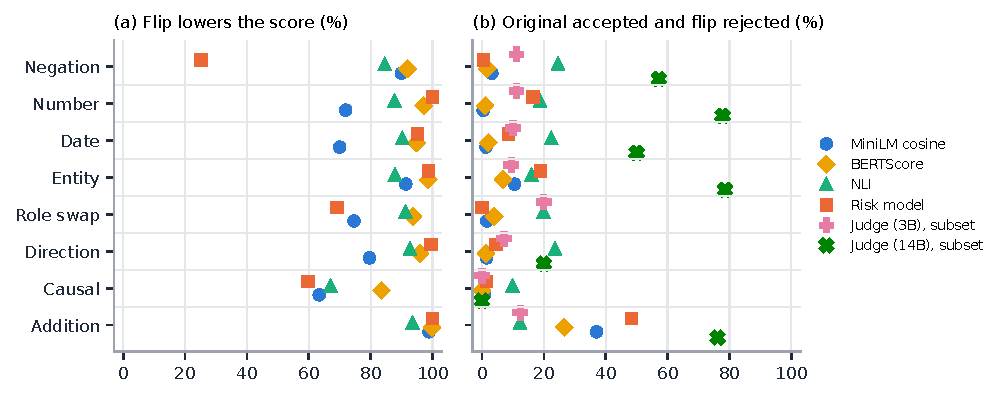
\includegraphics[width=\textwidth]{../figures/fig_cf_types.pdf}
\caption{Counterfactual sensitivity by perturbation type. (a) Share of flips that lower the score. (b) Paired detection: the unedited answer is accepted and the flip is rejected at the threshold fitted on natural calibration data.}
\label{fig:cftypes}
\end{figure*}

\paragraph{Scores move, decisions do not.} A single-fact flip lowers MiniLM's mean-max cosine in \CfCosDrop\% of pairs (Table~\ref{tab:cfdrop}), and the share is at least as high for BGE-small, BERTScore and NLI. Score-drop rates therefore make every method look sensitive. Decisions tell a different story (Figure~\ref{fig:cftypes}b, Table~\ref{tab:cfdetect}): with thresholds fitted on natural data, cosine accepts the unedited answer and rejects the flip in only \CfCosDetect\% \CfCosDetectCi\ of pairs. It rejects \CfCosFlipRej\% of flipped answers, but it accepts only \CfCosOrigAcc\% of the unedited faithful answers in the first place, so most rejections of flips are rejections the original would have received too. It accepts paraphrases about as often as the originals (\CfCosParaAcc\% vs.\ \CfCosParaOrigAcc\%), and among paraphrases whose original was accepted it rejects only \CfCosParaFalseRej\%. The descriptive half of H1 therefore holds: cosine is stable under rewording and rarely turns an accepted answer into a rejected one when a fact is changed. Paired detection is \CfNliDetect\% for NLI, \CfRiskDetect\% for the full risk model and \CfRiskChkDetect\% for the cosine-plus-checks variant; NLI exceeds cosine by \HoneNliMinusCos\ points \HoneNliMinusCosCi\ (Holm-adjusted $p\HoneNliHolm$).

The preregistered judge contrast of H1 uses the small judge (\CfJSmallN\ pairs, \CfJSmallBases\ bases; Table~\ref{tab:cfjudge}). It rejects \CfJSmallFlipRej\% of flips but accepts only \CfJSmallOrigAcc\% of originals, so its paired detection (\CfJSmallDetect\%) does not differ from cosine's (\HoneJudgeMinusCos\ points \HoneJudgeMinusCosCi, Holm-adjusted $p\HoneJudgeHolm$): H1 holds against NLI but not against the small judge. In an exploratory run (\CfJStrongN\ pairs, \CfJStrongBases\ bases, mostly additions, entities and negations), the 14B judge detects \CfJStrongDetect\% \CfJStrongDetectCi, \CfJStrongMinusCos\ points more than cosine \CfJStrongMinusCosCi\ and \CfJStrongMinusNli\ more than NLI \CfJStrongMinusNliCi\ on the same pairs---the only evaluator whose decisions track single-fact edits.

\paragraph{Inversion isolates sensitivity to the fact.} The paired detection rate is bounded by how often the original is accepted, and the score-drop rate rewards any change of wording. The inversion rate avoids both: holding the sentence, the evidence and the rest of the answer fixed, it asks whether the factual error scores at least as high as a harmless paraphrase. Here the methods separate sharply. NLI inverts in \CfNliInv\% \CfNliInvCi\ of triplets, MiniLM and BGE-small cosine in \CfCosInv\% and \CfBgeInv\%, BERTScore in \CfBertInv\%, the full risk model in \CfRiskInv\% and token precision in \CfTokPrecInv\%; MiniLM min-max cosine, which is driven by the least-supported sentence, inverts in most triplets. For a cosine score a paraphrase and a factual error are close to interchangeable, and the distributions of their score changes overlap almost completely (Figure~\ref{fig:locus}a).

\begin{figure*}[t]
\centering
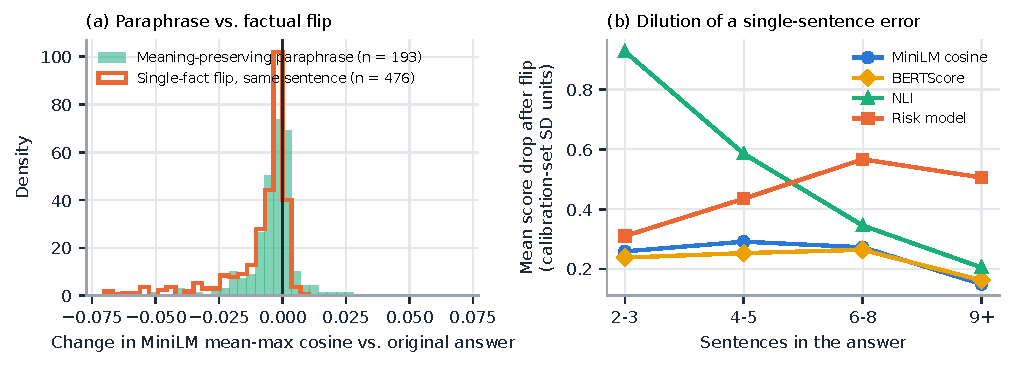
\includegraphics[width=\textwidth]{../figures/fig_locus.pdf}
\caption{(a) Change in MiniLM mean-max cosine caused by a meaning-preserving paraphrase and by a single-fact flip of the same sentence. (b) Mean score drop caused by a flip, in calibration-set standard deviations, by the number of sentences in the answer.}
\label{fig:locus}
\end{figure*}

\paragraph{Error types differ (H2).} Detection depends on the type of edit for every evaluator (within-base permutation test, $p\HtwoCosPerm$ for each; Cram\'er's $V$ from \CfNliCramerV\ for NLI to \CfRiskCramerV\ for the risk model). Unsupported additions are the only edit that cosine detects with any regularity (\CfCosDetectAddition\% paired detection); for numbers, dates, causal connectives and direction words its paired detection is \CfCosDetectNumber\%, \CfCosDetectDate\%, \CfCosDetectCausal\% and \CfCosDetectDirection\%. NLI is the most uniform across types (\CfNliDetectCausal\% to \CfNliDetectNegation\%) and the only method with substantial negation detection (\CfNliDetectNegation\%, against \CfCosDetectNegation\% for MiniLM). The explicit number and entity checks raise the risk model's detection of number and entity flips (\CfRiskDetectNumber\% and \CfRiskDetectEntity\%) but not of negation: a negation flip lowers the full model's support score in only \CfRiskDropNegation\% of pairs. Its strongest inputs barely react to negation---token precision falls for only \CfTokPrecDropNegation\% of negation flips, since words such as ``not'' usually occur somewhere in the evidence---and the weight it learned on the negation-mismatch feature is small and negative (Table~\ref{tab:coef}). A feature-based detector inherits the error distribution of its training labels.

\paragraph{Dilution.} Because cosine and NLI average over answer sentences, a fixed one-sentence error matters less in a longer answer (Figure~\ref{fig:locus}b). For NLI the mean drop falls from \CfNliDilFirst\ to \CfNliDilLast\ calibration standard deviations between the shortest and the longest answers; cosine's drop is small at every length (\CfCosDilFirst\ to \CfCosDilLast). The risk model, which includes per-sentence minima and counts of unsupported numbers and entities, does not dilute in the same way.

\subsection{Threshold transfer (RQ3)}
\label{sec:res-transfer}

\begin{figure*}[t]
\centering
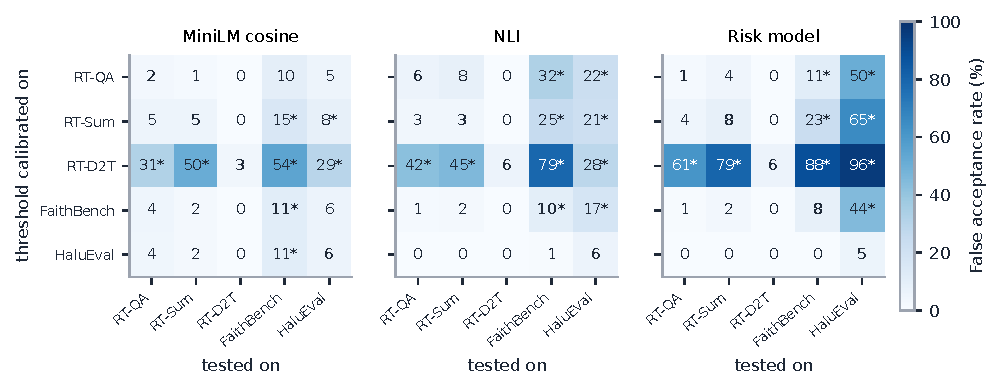
\includegraphics[width=\textwidth]{../figures/fig_transfer.pdf}
\caption{False-acceptance rate (\%) on the test split of the column domain when the threshold is calibrated to $\mathrm{FAR}\le5\%$ on the row domain. Bold: in-domain cells. *: the lower 95\% bound exceeds 5\%.}
\label{fig:transfer}
\end{figure*}

A threshold calibrated to $\mathrm{FAR}\le5\%$ mostly holds in its own domain: only \TrCosDiagExceed\ of the five diagonal cosine cells, FaithBench, has a lower confidence bound above 5\% (FAR \TrCosDiagMax\%), and the other in-domain cells stay close to the budget (Figure~\ref{fig:transfer}). The other evaluators behave similarly in-domain (one or two exceeding cells each, all below 14\%), except the full risk model, which has none. Across domains it does not. For MiniLM cosine \HthreeExceed\ of \HthreeCells\ off-diagonal cells exceed 5\% with the lower bound above 5\%, up to \TrCosOffMax\%, which supports H3 by the preregistered criterion (Bonferroni-adjusted bootstrap $p=\HthreePBonf$). The failure is not specific to cosine: the corresponding counts are \TrBgeOffExceed\ for BGE-small, \TrBertOffExceed\ for BERTScore, \TrNliOffExceed\ for NLI and \TrRiskOffExceed\ for the risk model, whose worst cell reaches \TrRiskOffMax\%. Thresholds learned on RT-D2T, where two thirds of answers are unsupported and support scores are low throughout, are the most permissive elsewhere; thresholds learned on FaithBench and HaluEval-QA are conservative on RAGTruth. Within RAGTruth, a threshold calibrated on long answers and applied to short ones raises cosine FAR to \ShLenCosLongToShort\% and the risk model's to \ShLenRiskLongToShort\%, whereas changing the generator family moves FAR by a few points only (Table~\ref{tab:shift}). Calibrated probabilities do not transfer either: the risk model's expected calibration error is \CalQaEce\ on RT-QA but \CalFbEce\ on FaithBench and \CalHaluEce\ on HaluEval-QA.

\subsection{Selective evaluation (RQ4)}
\label{sec:res-cascade}

\paragraph{Cheap stage.} On the full RAGTruth test set at $\alpha=0.05$ and $\beta=0.10$ (Table~\ref{tab:cheapstage}), the cosine gate resolves \CsCosFiveCov\% \CsCosFiveCovCi\ of answers without a judge, with a cheap-stage FAR of \CsCosFiveFar\%. The full risk model resolves \CsRiskFiveCov\% \CsRiskFiveCovCi\ at a cheap-stage FAR of \CsRiskFiveFar\%, \HfourRiskDiff\ points more than cosine \HfourRiskDiffCi\ (Holm-adjusted $p\HfourHolm$); NLI and BGE-small resolve \HfourNliDiff\ and \HfourBgeDiff\ points more than MiniLM. The cosine-plus-checks variant does not resolve more than cosine (\HfourRiskChkDiff\ points, \HfourRiskChkDiffCi). Within domain the calibration-time FAR budget is approximately met by every gate; on FaithBench, with thresholds carried over from RT-Sum, the cheap-stage FAR rises to \FbOodCosFar\% for cosine and \FbOodRiskFar\% for the risk model.

\begin{table*}[t]
\centering\small
\resizebox{\textwidth}{!}{\begin{tabular}{llrlrrlr}
\toprule
Policy & Gate & Judged\,\% & BAcc [95\% CI] & FAR\,\% & FRR\,\% & $\Delta$BAcc vs.\ always-judge & Random \\
\midrule
Always judge & -- & 100.0 & .566 [.543, .592] & 1.6 & 85.2 & -- & -- \\
\midrule
Never judge & Token precision & 0.0 & .569 [.516, .627] & 48.1 & 38.1 & .004 [-.051, .063] & -- \\
Never judge & MiniLM cosine (mean-max) & 0.0 & .625 [.581, .667] & 33.3 & 41.8 & .059 [.015, .100] & -- \\
Never judge & BGE-small cosine (mean-max) & 0.0 & .559 [.513, .603] & 41.0 & 47.2 & -.006 [-.057, .041] & -- \\
Never judge & BERTScore & 0.0 & .567 [.514, .617] & 49.2 & 37.5 & .001 [-.055, .056] & -- \\
Never judge & NLI (SummaC-ZS style) & 0.0 & .585 [.538, .631] & 34.4 & 48.6 & .019 [-.030, .068] & -- \\
Never judge & Risk model: full & 0.0 & .634 [.583, .681] & 36.1 & 37.2 & .068 [.017, .117] & -- \\
\midrule
Gate, $\alpha=0.05$ & MiniLM cosine (mean-max) & 75.9 & .581 [.550, .613] & 7.1 & 76.7 & .015 [-.009, .041] & .579 \\
Gate, $\alpha=0.05$ & NLI (SummaC-ZS style) & 73.3 & .583 [.551, .616] & 10.9 & 72.4 & .017 [-.009, .045] & .571 \\
Gate, $\alpha=0.05$ & Risk model: cosine + checks & 77.9 & .595 [.566, .625] & 4.4 & 76.7 & .029 [.007, .051] & .596 \\
Gate, $\alpha=0.05$ & Risk model: full & 64.5 & .635 [.601, .671] & 7.7 & 65.3 & .069 [.039, .101] & .589 \\
\midrule
Gate, $\alpha=0.1$ & MiniLM cosine (mean-max) & 67.1 & .594 [.559, .627] & 13.1 & 68.2 & .028 [-.004, .060] & .587 \\
Gate, $\alpha=0.1$ & NLI (SummaC-ZS style) & 63.4 & .608 [.573, .643] & 16.4 & 61.9 & .043 [.013, .072] & .572 \\
Gate, $\alpha=0.1$ & Risk model: cosine + checks & 67.9 & .631 [.599, .665] & 8.7 & 65.1 & .065 [.036, .094] & .610 \\
Gate, $\alpha=0.1$ & Risk model: full & 58.3 & .664 [.629, .699] & 8.7 & 58.5 & .098 [.066, .132] & .595 \\
\midrule
Gate, $\alpha=0.2$ & MiniLM cosine (mean-max) & 53.8 & .625 [.585, .663] & 20.2 & 54.8 & .059 [.020, .096] & .593 \\
Gate, $\alpha=0.2$ & NLI (SummaC-ZS style) & 49.2 & .619 [.577, .659] & 27.3 & 48.9 & .053 [.014, .093] & .576 \\
Gate, $\alpha=0.2$ & Risk model: cosine + checks & 53.1 & .643 [.605, .681] & 19.1 & 52.3 & .077 [.040, .113] & .631 \\
Gate, $\alpha=0.2$ & Risk model: full & 41.1 & .678 [.636, .720] & 21.9 & 42.6 & .112 [.070, .153] & .607 \\
\bottomrule
\end{tabular}
}
\caption{System results on the RAGTruth and FaithBench judged subset ($n=\SysSmallN$) with the small judge. ``Judged'' is the share escalated; ``Random'' is the mean balanced accuracy when the same number of randomly chosen examples is escalated and the rest decided by the gate's $\tau^\mathrm{bal}$.}
\label{tab:cascadesmall}
\end{table*}

\paragraph{System.} With the small judge (Table~\ref{tab:cascadesmall}), always judging gives a balanced accuracy of only \SysSmallJudgeBacc\ on the judged subset, because the judge rejects most faithful answers. Every cascade is at least as good, and the risk-gated cascade at $\alpha=0.05$ is \SysSmallRiskFiveDiff\ \SysSmallRiskFiveDiffCi\ better while sending \SysSmallRiskFiveEsc\% of examples to the judge; random escalation of the same share gives \SysSmallRiskFiveRand. The second condition of H4 (no more than two points below always-judge) is therefore met, but trivially, because the reference point is weak; the escalation curves (Figure~\ref{fig:escalation}) show that with this judge the best policy escalates only a small share of examples, and that escalating the smallest-margin examples first beats random escalation clearly for the risk model, slightly for NLI and not at all for cosine.

With the 14B judge on its \SysStrongN\ RAGTruth answers (Table~\ref{tab:cascadestrong}), the ordering reverses. Judging everything gives \SysStrongJudgeBacc\ \SysStrongJudgeBaccCi, and every cheap method alone is worse (cosine \SysStrongNeverCosDiff\ \SysStrongNeverCosDiffCi, full risk model \SysStrongNeverRiskDiff\ \SysStrongNeverRiskDiffCi). The cascades now trade accuracy for judge calls. The cosine gate at $\alpha=0.05$ skips \SysStrongCosFiveSaved\% of judge calls at \SysStrongCosFiveDiff\ \SysStrongCosFiveDiffCi; the risk gate skips \SysStrongRiskFiveSaved\% at \SysStrongRiskFiveDiff\ \SysStrongRiskFiveDiffCi; the cosine-plus-checks gate skips \SysStrongRiskChkFiveSaved\% at \SysStrongRiskChkFiveDiff\ \SysStrongRiskChkFiveDiffCi. The intervals include both no loss and losses well beyond the two-point margin of H4, so on this subset the accuracy condition of H4 can be neither confirmed nor rejected for the stronger judge. Targeted escalation still beats random escalation of the same share for the risk gate (\SysStrongRiskFiveBacc\ vs.\ \SysStrongRiskFiveRand).

\begin{figure*}[t]
\centering
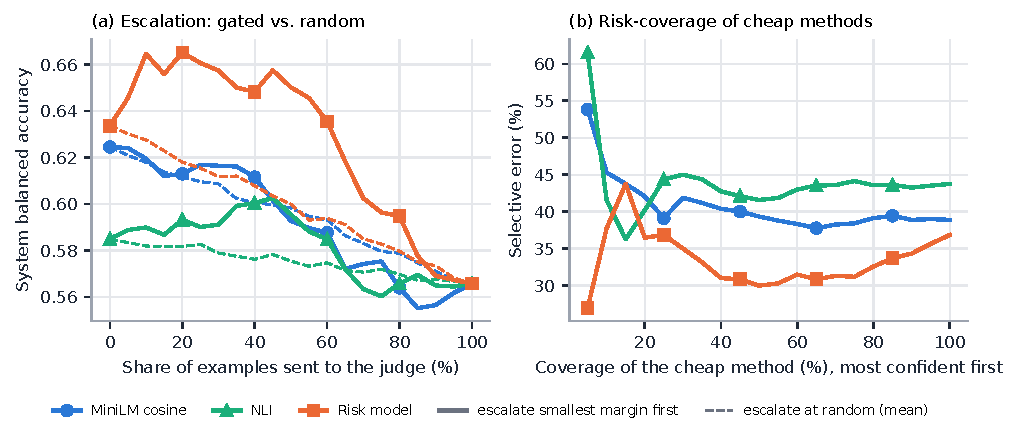
\includegraphics[width=\textwidth]{../figures/fig_escalation.pdf}
\caption{(a) System balanced accuracy on the small-judge subset as a function of the share escalated, escalating the smallest-margin examples first (solid) or at random (dashed, mean over draws). (b) Risk--coverage curves of the cheap methods alone.}
\label{fig:escalation}
\end{figure*}

\paragraph{Correctness.} On the full EVOUNA-NQ test set the reference-mode risk model resolves \EvCsRiskCov\% of answers at a cheap-stage FAR of \EvCsRiskFar\%. On the 600 judged answers it escalates \EvCsRiskEsc\% to the small judge, and the system reaches a balanced accuracy of \EvCsRiskSysBacc; the cosine-gated system escalates \EvCsCosEsc\% and reaches \EvCsCosSysBacc.

\subsection{Cost (RQ5)}
\label{sec:cost}

\begin{table*}[t]
\centering\small
\resizebox{\textwidth}{!}{\begin{tabular}{lrrrrrrr}
\toprule
Method & Median ms & p95 ms & Wall s / 1k & CPU s / 1k & Cold start s & Prompt tok. & Out tok. \\
\midrule
Lexical features + checks & 1.4 & 2.8 & 1.5 & 2 & 0.0 & -- & -- \\
MiniLM cosine & 321 & 1,083 & 433 & 2,574 & 6.4 & -- & -- \\
\quad evidence embeddings cached & 42.9 & 83.2 & 49.1 & 292 & 6.4 & -- & -- \\
BGE-small cosine & 631 & 2,046 & 831 & 4,934 & 1.8 & -- & -- \\
\quad evidence embeddings cached & 85.1 & 163 & 95.6 & 562 & 1.8 & -- & -- \\
Risk model: full & 414 & 1,164 & 513 & 3,046 & 6.4 & -- & -- \\
\midrule
BERTScore (roberta-base) & 1,005 & 1,945 & 1,039 & 6,122 & 1.7 & -- & -- \\
NLI (DeBERTa-v3-base) & 2,302 & 5,865 & 2,900 & 15,206 & 9.7 & -- & -- \\
\midrule
Judge (3B), new source & 10,292 & 23,181 & 11,791 & -- & 4.4 & 861 & 9.0 \\
\quad same source (prefix cached) & 4,711 & 5,955 & 4,736 & -- & 4.4 & 839 & 9.0 \\
\midrule
Judge (14B), new source & 38,475 & 95,366 & 46,463 & -- & 15.7 & 867 & 10.1 \\
\quad same source (prefix cached) & 13,547 & 19,472 & 13,953 & -- & 15.7 & 846 & 9.4 \\
\bottomrule
\end{tabular}
}
\caption{Measured cost on one CPU-only laptop (\HwCores\ logical cores, \HwRam\,GB RAM, \HwThreads\ PyTorch threads, no GPU), on a fixed sample of \CostSampleN\ RAGTruth answers (mean \CostAnsWords\ answer words, \CostEvWords\ evidence words), single process, no other job running. Wall and CPU seconds per 1{,}000 evaluations exclude cold start, which is reported separately. Judge rows: 30 calls each; ``prefix cached'' is a second answer for the same source, for which the server reuses the cached evidence prefix. No paid API was used, so no monetary cost is reported.}
\label{tab:cost}
\end{table*}

\begin{figure*}[t]
\centering
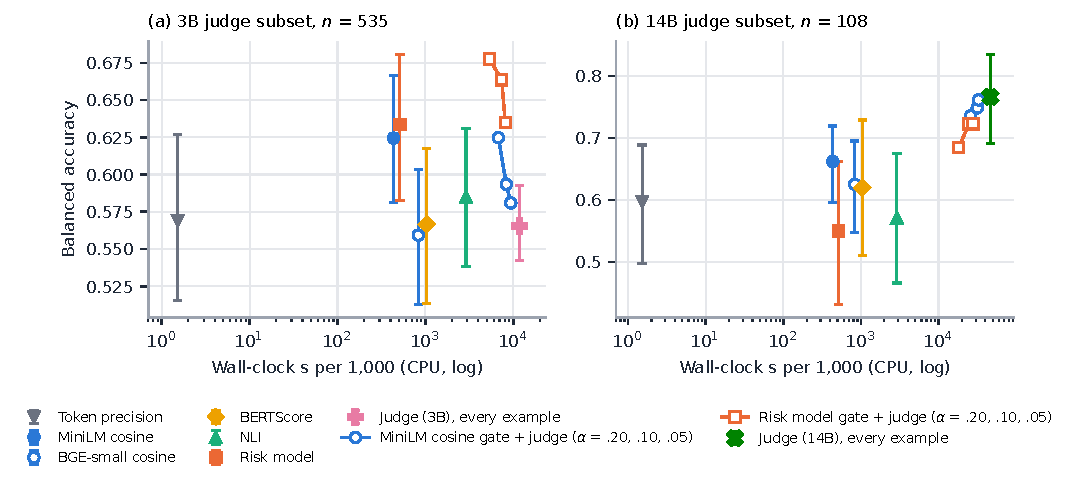
\includegraphics[width=\textwidth]{../figures/fig_pareto.pdf}
\caption{Balanced accuracy against measured wall-clock cost per 1{,}000 evaluations on the two judged subsets. Cascade cost is the cheap-stage cost for every example plus the judge cost for the escalated share. Error bars: 95\% cluster-bootstrap intervals. The panels use different examples and are not directly comparable.}
\label{fig:pareto}
\end{figure*}

Table~\ref{tab:cost} reports measured cost. Lexical features with the number and entity checks take \CostLexicalAndChecksWall\,s per 1{,}000 answers. MiniLM cosine takes \CostMinilmCosineWall\,s including evidence encoding and \CostMinilmCosineEvidenceCachedWall\,s when evidence embeddings are cached; the full risk model, which needs MiniLM embeddings, takes \CostRiskFullWall\,s. Relative to MiniLM cosine with evidence encoding, BERTScore costs \CostBertscoreRatio$\times$, NLI \CostNliRatio$\times$, the 3B judge \CostJudgeSmallRatio$\times$ (\CostJudgeSmallPrefixCachedRatio$\times$ when the evidence prefix is cached) and the 14B judge \CostJudgeStrongRatio$\times$ (\CostJudgeStrongPrefixCachedRatio$\times$). Judge cost is dominated by reading the prompt (about \CostJudgeSmallPtok\ tokens, processed at \CostJudgeSmallTokPerS\ tokens/s by the 3B and \CostJudgeStrongTokPerS\ tokens/s by the 14B model), which is why prefix caching helps so much when several answers share one source.

Figure~\ref{fig:pareto} combines cost with accuracy. With the 3B judge, the risk gate is better and cheaper than judging everything at every $\alpha$; at $\alpha=0.20$ it reaches \SysSmallRiskTwentyBacc\ while judging \SysSmallRiskTwentyEsc\% of examples. With the 14B judge, every cheap method alone is far below the judge, and the gates save between a quarter and two fifths of judge time at an accuracy cost that this subset cannot pin down. These cost figures are specific to one CPU laptop; we did not measure GPU inference, where the ratios between methods may differ.

\section{Discussion}
\label{sec:discussion}

\paragraph{When is cosine enough?} On our evidence, rarely as a decision rule and never as a guarantee. Cosine detects one kind of error with some reliability---content that has no counterpart in the evidence---the most common annotated hallucination type in RAGTruth. It does not detect changed numbers, dates, causal connectives, directions or negations: for these, its paired detection is close to zero, and in more than a third of matched triplets the edit scores at least as high as a paraphrase of the same sentence. In its best configuration it ranks natural answers no better than token overlap with the evidence, and inside a feature model it adds no information beyond lexical features. Its one practical virtue is stability: it rarely rejects a harmless rewording, so a cosine gate that \emph{accepts} only very high-similarity answers wastes little. It is also cheap enough to compute everywhere. The defensible uses are therefore narrow: a first-pass filter for answers that are near-copies of their evidence, a feature among others, or a monitoring signal for gross drift---not a factuality check.

\paragraph{Score movement is not detection.} Every method in our study lowers its score for most single-fact flips, and a study that reported only score drops would conclude that all of them are sensitive. What matters in deployment is whether a fixed threshold changes its decision, and against that criterion detection rates are several times lower (for cosine, \CfCosDrop\% score drops but \CfCosDetect\% paired detection). The inversion rate makes the reason visible: cosine's response to a factual edit is the same size as its response to a paraphrase, so the threshold cannot separate them. We recommend that perturbation studies of factuality metrics report a matched paraphrase control and a decision-level metric alongside score drops.

\paragraph{NLI is the most fact-sensitive cheap method, but not the best ranker.} A zero-shot NLI scorer has the lowest inversion rate by a wide margin and the most uniform detection across error types, yet on natural RAGTruth data it is no better than cosine at its calibrated threshold. Its sensitivity is diluted by sentence averaging in long answers, and its thresholds transfer no better than anyone else's. Trained grounding detectors \citep{tang2024minicheck,zha2023alignscore} are the obvious next step and may change this picture.

\paragraph{Thresholds are the weak point.} The most consistent result of the study is that a calibrated false-acceptance budget is a property of a threshold \emph{and} a distribution. Every evaluator, including the learned risk model, stayed near a 5\% budget in-domain and broke it in several other domains, by up to an order of magnitude; within one benchmark, answer length alone was enough. Any deployment that uses a fixed similarity threshold should recalibrate it per domain on labelled data; the acceptance rate alone is not a reliable alarm, because in several failing transfer cells it moved by only a few points (Table~\ref{tab:transfermatrix}).

\paragraph{Cascades help only as much as the judge.} A cheap risk score resolves more examples than cosine within an error budget, but what that buys depends on the judge. With the 3B judge the cascade mainly \emph{protected} the system from the judge; with the 14B judge it saved a quarter to two fifths of judge calls at an accuracy cost our subset could not pin down. Because the 14B judge was strict on some tasks and lenient on summaries, a judge can fail in either direction, and it needs its own validation and calibration on the target distribution before a cascade is built around it. The random-escalation control is essential for reading these results: only the risk model's margin made targeted escalation clearly better than random.

\section{Ablations and Error Analysis}
\label{sec:ablation}

\begin{table}[t]
\centering\small
\setlength{\tabcolsep}{2.5pt}
\resizebox{\columnwidth}{!}{\begin{tabular}{lrlrrrr}
\toprule
 & \multicolumn{2}{c}{RAGTruth test AUC} & FaithB. & HaluEval & \multicolumn{2}{c}{Counterfactual} \\
Feature set & AUC & $\Delta$ vs.\ full [95\% CI] & AUC & AUC & drop\,\% & AUC \\
\midrule
All groups (full) & .817 &  & .637 & .977 & 79.4 & .606 \\
\midrule
$-$ cosine & .818 & .000 [-.002, .003] & .644 & .983 & 79.4 & .612 \\
$-$ lexical & .794 & -.023 [-.033, -.014] & .583 & .693 & 89.8 & .639 \\
$-$ number & .812 & -.005 [-.009, -.002] & .633 & .976 & 79.3 & .592 \\
$-$ entity & .810 & -.008 [-.012, -.003] & .633 & .974 & 79.0 & .573 \\
$-$ negation & .816 & -.001 [-.002, .000] & .642 & .978 & 93.1 & .608 \\
$-$ length & .808 & -.010 [-.015, -.005] & .644 & .965 & 76.7 & .607 \\
\midrule
only cosine & .746 &  & .535 & .244 & 83.4 & .580 \\
only lexical & .789 &  & .637 & .973 & 88.6 & .551 \\
only number & .565 &  & .504 & .560 & 22.3 & .597 \\
only entity & .663 &  & .581 & .719 & 39.3 & .652 \\
only negation & .547 &  & .580 & .533 & 26.5 & .563 \\
only length & .661 &  & .597 & .975 & 47.8 & .555 \\
\bottomrule
\end{tabular}
}
\caption{Feature-group ablation of the full risk model (logistic regression, RAGTruth training split). $\Delta$: AUC change on the RAGTruth test split when the group is removed, with a 95\% cluster-bootstrap interval. ``Counterfactual'': share of flips that lower the support score, and AUC for separating originals from flips.}
\label{tab:ablation}
\end{table}

\paragraph{Cosine adds nothing on top of lexical grounding.} Removing the three cosine features from the full risk model leaves its RAGTruth test AUC unchanged (\AblMinusCosineLoss\ \AblMinusCosineLossCi; Table~\ref{tab:ablation}), whereas removing the lexical group costs \AblMinusLexicalLoss\ \AblMinusLexicalLossCi\ and is the largest loss. On its own the lexical group (AUC \AblOnlyLexicalAuc) beats the cosine group (\AblOnlyCosineAuc). The number, entity and length groups each contribute a small but reliable amount; the negation group contributes nothing measurable on natural data. A gradient-boosted model on the same features gives similar AUCs (RT-QA \GbmQaAuc\ vs.\ \LrQaAuc\ for logistic regression), so the conclusion does not depend on the linear form.

\paragraph{What the risk model learns.} The largest standardised coefficients (Table~\ref{tab:coef}) are answer length (longer answers are riskier) and token precision; MiniLM document cosine enters with a \emph{positive} risk coefficient once lexical features are present, i.e.\ it is used as a correction term rather than as evidence of support. Length is a legitimate signal on RAGTruth---longer answers have more opportunities to add unsupported material---but it is also what makes the model's thresholds fragile under length shift (Section~\ref{sec:res-transfer}) and what lets it reach near-perfect AUC on HaluEval-QA for reasons unrelated to grounding.

\paragraph{Natural versus counterfactual sensitivity.} Feature groups that matter on natural data and on counterfactuals are different. Dropping the lexical group lowers natural AUC but \emph{raises} the share of flips that lower the score (Table~\ref{tab:ablation}), and the entity group alone separates originals from flips better (counterfactual AUC \AblOnlyEntityCfAuc) than the full model (\AblFullCfAuc). Natural benchmarks reward features that track the prevalent kind of hallucination in their generators---mostly added, unsupported content---and are nearly silent about value substitutions inside an otherwise grounded sentence, which is exactly where cosine fails.

\section{Limitations and Threats to Validity}
\label{sec:limitations}

\paragraph{Judge scale.} Both LLM judges were run on fixed, source-clustered subsets rather than on full test sets, because a CPU-only machine evaluates a 14B model at seconds to tens of seconds per call. Judge intervals are correspondingly wide, comparisons between a judge and a cheap evaluator are made only on the judged subset, and cascade system metrics are reported on those subsets. The judges are two open-weight models with one main rubric; our results say nothing about frontier API judges, which may behave differently. The prompt-sensitivity check covers one alternative rubric for the small judge only.

\paragraph{Counterfactual labels.} The flips are produced by rules and checked by rules: the replaced value must occur in the evidence and the replacement must not. Some flips will nevertheless be wrong (an entity replacement that the evidence happens to support under another name, a negation that yields an awkward but still entailed sentence), and some paraphrases may change meaning despite the filters. A 160-pair audit sheet is released but no human has reviewed it, so every counterfactual number is a measurement against rule-generated labels. Edits are single-sentence and single-fact; they are cleaner than natural hallucinations and should be read as a diagnostic of sensitivity, not as an estimate of field error rates.

\paragraph{Datasets.} RAGTruth responses come from 2023-era generators, FaithBench is small and deliberately hard (it collects summaries on which earlier detectors disagree), HaluEval-QA labels are synthetic and its hallucinated answers differ from correct ones in length and style, and EVOUNA-NQ measures agreement with short reference answers. FactBench was not used. The transfer matrix therefore spans five domains with very different base rates; a FAR exceedance on one of them may reflect label construction as much as evaluator behaviour.

\paragraph{Evaluator coverage.} We use one NLI checkpoint in a zero-shot SummaC-style configuration and do not evaluate trained grounding detectors such as MiniCheck or AlignScore \citep{tang2024minicheck,zha2023alignscore}, which may close much of the gap to the judges at moderate cost. A third embedding model planned in advance was not run (Appendix~\ref{app:deviations}). The risk estimator is a linear model on hand-built features fitted on RAGTruth training data; it inherits RAGTruth's notion of a hallucination.

\paragraph{Statistics.} Cluster bootstrap intervals treat source documents as independent, and the Holm correction covers only the preregistered primary family; the many secondary comparisons in the tables are descriptive. Calibration-time guarantees for the cascade hold only for data exchangeable with the calibration split.

\paragraph{Cost.} Latency was measured on one laptop CPU with batch sizes chosen for that machine. Absolute times, and probably the ratios between methods, will differ on a GPU or with a hosted API; we did not measure either. No commercial API was used, so no dollar costs are reported.


\section{Conclusion}
\label{sec:conclusion}

Embedding cosine is rarely enough to judge factuality. It ranks faithfulness no better than lexical overlap, adds nothing to a feature model, is weaker than reference containment on correctness, and responds to a single changed fact about as much as to a harmless paraphrase, so thresholds fitted on natural data rarely turn an accepted answer into a rejected one. NLI is more sensitive to the fact itself, and a cheap risk score resolves more examples within an error budget, but no threshold survived a change of domain. LLM judges were not a safe default either. A 3B judge failed on long evidence. A 14B judge was the only evaluator that tracked single-fact edits, but it was lenient on summaries and cost \CostJudgeStrongRatio\ times as much as cosine. We recommend treating cosine as one weak feature, testing metrics with matched paraphrase controls and decision-level metrics, and recalibrating thresholds and judges wherever the data change. Code, configurations, raw judge outputs and analysis outputs are available at \CodeURL.


\section*{Use of AI Assistance}
The experimental pipeline, analyses and manuscript were produced with substantial assistance from an AI coding agent (Claude, Anthropic) working under the author's direction. All experiments were actually run, and every reported number is generated by script from the released result files. The author reviewed the work and takes full responsibility for its content.

\bibliography{references}

\appendix
\section{Judge Prompts}
\label{app:prompts}

The system message is one of the rubrics below, reproduced verbatim from \texttt{src/run\_judge.py}. In evidence mode the user message is ``\texttt{EVIDENCE:} \emph{evidence}'', then ``\texttt{QUESTION:} \emph{question}'' when one exists, then ``\texttt{ANSWER:} \emph{answer}'' (``\texttt{SOURCE}''/``\texttt{RESPONSE}'' for the v2 variant). In reference mode it is the question, a bulleted list of reference answers and the candidate answer. Placing the evidence before the answer lets consecutive calls for one source share a prompt prefix. Output is constrained to the JSON schema \texttt{\{"verdict": enum\}}. Options: temperature 0, seed \Seed, context 6{,}144 tokens, at most 24 output tokens. The probability of \textsc{supported} is read from the token distribution at the first token of the verdict string and is used only for the judges' AUC and score-drop statistics.

\paragraph{Evidence-grounded rubric (primary, v1).}
\begin{quote}\small\ttfamily\raggedright
You are a strict fact-checking judge. You receive EVIDENCE, sometimes a QUESTION, and an ANSWER. Decide whether every factual claim in the ANSWER is supported by the EVIDENCE.\\
- SUPPORTED: every factual claim in the answer is stated in, or directly entailed by, the evidence. Paraphrasing is fine.\\
- UNSUPPORTED: at least one claim contradicts the evidence (for example a wrong number, date, name, negation, cause, or who did what to whom).\\
- INSUFFICIENT\_EVIDENCE: no claim contradicts the evidence, but at least one claim adds information that the evidence does not contain.\\
Judge only against the evidence, never from your own knowledge. Ignore style, fluency and completeness.\\
Reply with one JSON object: \{\textquotedbl{}verdict\textquotedbl{}: \textquotedbl{}SUPPORTED\textquotedbl{} | \textquotedbl{}UNSUPPORTED\textquotedbl{} | \textquotedbl{}INSUFFICIENT\_EVIDENCE\textquotedbl{}\}
\end{quote}
\paragraph{Evidence-grounded rubric (sensitivity variant, v2).}
\begin{quote}\small\ttfamily\raggedright
Task: hallucination check. Read the SOURCE material and the RESPONSE written from it. A response is faithful only if a careful reader could verify each of its statements from the source alone.\\
Choose one label:\\
SUPPORTED = the response is fully faithful to the source.\\
UNSUPPORTED = the response states something that conflicts with the source.\\
INSUFFICIENT\_EVIDENCE = nothing conflicts, but the response includes details absent from the source.\\
Do not use outside knowledge. Do not penalise wording or omissions.\\
Answer with JSON only: \{\textquotedbl{}verdict\textquotedbl{}: \textquotedbl{}<label>\textquotedbl{}\}
\end{quote}
\paragraph{Reference-based rubric (EVOUNA-NQ).}
\begin{quote}\small\ttfamily\raggedright
You are a strict grader of answers to factual questions. You receive a QUESTION, one or more REFERENCE ANSWERS (any one of them is correct) and a CANDIDATE ANSWER.\\
- SUPPORTED: the candidate gives the same answer as a reference. Different wording and extra correct detail are fine.\\
- UNSUPPORTED: the candidate gives a different or conflicting answer, or does not answer the question.\\
- INSUFFICIENT\_EVIDENCE: the references do not let you decide whether the candidate is right.\\
Grade only against the references, never from your own knowledge.\\
Reply with one JSON object: \{\textquotedbl{}verdict\textquotedbl{}: \textquotedbl{}SUPPORTED\textquotedbl{} | \textquotedbl{}UNSUPPORTED\textquotedbl{} | \textquotedbl{}INSUFFICIENT\_EVIDENCE\textquotedbl{}\}
\end{quote}


\section{Configuration}
\label{app:config}

\begin{itemize}\setlength{\itemsep}{0pt}
\item Seed \Seed\ for all sampling and decoding; \NBoot\ bootstrap resamples.
\item Embedders: \nolinkurl{sentence-transformers/all-MiniLM-L6-v2}, \nolinkurl{BAAI/bge-small-en-v1.5}; unit-normalised; at most 40 answer sentences and 400 evidence chunks per example.
\item BERTScore: \nolinkurl{FacebookAI/roberta-base}, layer 10, no IDF, no rescaling.
\item NLI: \nolinkurl{MoritzLaurer/DeBERTa-v3-base-mnli-fever-anli}, two retrieved chunks per answer sentence, maximum 320 tokens per pair.
\item Judges: Ollama tags \texttt{\JudgeSmallModel} and \texttt{\JudgeStrongModel}; model digests are recorded in \texttt{configs/experiment.yaml}.
\item Paraphraser: Ollama tag \texttt{phi4-mini:3.8b}; kept if numbers, capitalised tokens and negation parity are unchanged, the length ratio is in $[0.6,1.7]$ and token Jaccard similarity to the original sentence is at most $0.9$.
\item Risk estimator: \texttt{StandardScaler} + \texttt{LogisticRegression(C=1.0)}; isotonic calibration on the calibration split.
\item Cascade: $\alpha\in\{0.05,0.10,0.20\}$, $\beta=0.10$, thresholds per domain.
\end{itemize}

\section{Data Processing}
\label{app:data}

Sources and licences: RAGTruth (MIT), FaithBench (CC BY-NC-SA 4.0), EVOUNA from the QA-Eval repository (Apache-2.0), HaluEval (MIT), each downloaded from the authors' public repository; \texttt{data/README.md} gives the exact files and commands. RAGTruth evidence is the retrieved passages (QA), the article (Sum) or the JSON record flattened to ``key: value.''\ lines (D2T). EVOUNA gold answers are split on ``/'' into alternative references. Sentences are split with a regular expression that protects common abbreviations. Evidence chunks are windows of two consecutive sentences with stride one; sentences longer than 60 words are windowed. No example was removed on the basis of any evaluator's output.

\section{Departures from the Preregistered Plan}
\label{app:deviations}

\begin{enumerate}\setlength{\itemsep}{0pt}
\item \textbf{Third embedder dropped.} The plan named bge-base-en-v1.5. It could not be downloaded for lack of disk space, and the substitute (nomic-embed-text served by Ollama) encoded about six texts per second, too slow for \NTestNatural\ test examples plus counterfactuals. Two embedders are reported.
\item \textbf{Paraphrase model and count.} The paraphraser was changed from gemma3:4b to phi4-mini:3.8b and the number of bases from 450 to 240 for memory and time reasons, before any paraphrase was scored.
\item \textbf{Sentence splitter fix.} A bug that split sentences after abbreviations such as ``Dr.''\ was found while reading training-split counterfactuals. It was fixed and the counterfactual set was rebuilt before any evaluator was run on it.
\item \textbf{H2 test.} The permutation test shuffles outcomes among the pairs of one base response; a chi-square statistic and Cram\'er's $V$ are reported alongside it.
\item \textbf{H3 p-value.} The plan specified a confidence-interval criterion. To include H3 in the Holm family we additionally report a Bonferroni-adjusted one-sided bootstrap p-value over the 20 off-diagonal cells.
\item \textbf{Crash recovery and numeric precision.} The first embedding and BERTScore runs ran out of memory because the disk was full and an LLM was loaded at the same time; both were re-run alone, with BERTScore restructured to encode one evidence text at a time. The first NLI run loaded the checkpoint in its stored 16-bit precision, which was about thirteen times slower on this CPU; it was stopped before writing any score and re-run in 32-bit precision. None of these changes alters a score definition.
\item \textbf{Cost benchmark re-run.} The first clean benchmark crashed while summarising the judge rows because one judge call had returned no verdict; it saved nothing. The summary was changed to use successful calls and record failures, and the whole benchmark was re-run alone; all 120 judge calls in the reported run succeeded.
\item \textbf{Judge for H4.} The plan does not name the judge for H4. The confirmatory test uses the small judge, which has the larger subset; the 14B-judge cascade is reported as exploratory.
\item \textbf{No human audit.} The released 160-pair audit sheet has not been reviewed; no human validation of counterfactual labels is claimed.
\end{enumerate}

\section{Reproduction}
\label{app:repro}

{\footnotesize\ttfamily\raggedright\setlength{\parskip}{1pt}
\par\hangindent=1.5em\hangafter=1 pip install -r requirements.txt
\par\hangindent=1.5em\hangafter=1 python src/prepare\_data.py
\par\hangindent=1.5em\hangafter=1 python src/build\_counterfactuals.py -{}-split test
\par\hangindent=1.5em\hangafter=1 python src/build\_counterfactuals.py -{}-split test -{}-paraphrase
\par\hangindent=1.5em\hangafter=1 python src/score\_cheap.py -{}-skip-nomic
\par\hangindent=1.5em\hangafter=1 python src/run\_nli.py
\par\hangindent=1.5em\hangafter=1 python src/run\_bertscore.py
\par\hangindent=1.5em\hangafter=1 python src/run\_judge.py -{}-select
\par\hangindent=1.5em\hangafter=1 python src/run\_judge.py -{}-judge small -{}-part natural
\par\hangindent=1.5em\hangafter=1 python src/run\_judge.py -{}-judge small -{}-part cf
\par\hangindent=1.5em\hangafter=1 python src/run\_judge.py -{}-judge small -{}-part sensitivity -{}-prompt v2
\par\hangindent=1.5em\hangafter=1 python src/run\_judge.py -{}-judge strong -{}-part natural
\par\hangindent=1.5em\hangafter=1 python src/run\_judge.py -{}-judge strong -{}-part cf
\par\hangindent=1.5em\hangafter=1 python src/analyze.py
\par\hangindent=1.5em\hangafter=1 python src/cost\_benchmark.py -{}-strong
\par\hangindent=1.5em\hangafter=1 python src/make\_tables.py
\par\hangindent=1.5em\hangafter=1 python src/make\_figures.py
\par\hangindent=1.5em\hangafter=1 python src/lint\_paper.py\par}
\noindent Dataset download commands are in \texttt{data/README.md}; \texttt{README.md} gives a single command that runs the whole sequence. The judge scripts are resume-safe and require a local Ollama server with the two judge models and the paraphrase model pulled.

\section{Additional Results}
\label{app:more}

\begin{table*}[t]
\centering\small
\resizebox{\textwidth}{!}{\begin{tabular}{lrrrrrrrrrrr}
\toprule
Method & Neg. & Num. & Date & Entity & Role & Dir. & Causal & Add. & All & Orig.\ acc. & Para.\ acc. \\
$n$ pairs & 1432 & 773 & 540 & 1018 & 126 & 466 & 273 & 1517 & 6145 & 6145 & 193 \\
\midrule
Token precision & 0.5 & 3.1 & 1.9 & 6.6 & 0.0 & 2.8 & 1.5 & 33.9 & 10.4 & 65.3 & 49.2 \\
MiniLM cosine (document) & 1.0 & 0.3 & 0.4 & 13.8 & 4.8 & 1.1 & 0.4 & 15.4 & 6.6 & 61.9 & 46.6 \\
MiniLM cosine (mean-max) & 3.2 & 0.4 & 1.3 & 10.5 & 1.6 & 1.5 & 0.7 & 37.0 & 12.0 & 57.8 & 56.0 \\
MiniLM cosine (min-max) & 0.4 & 0.0 & 0.0 & 4.0 & 0.0 & 0.4 & 0.4 & 55.6 & 14.5 & 69.8 & 72.5 \\
BGE-small cosine (mean-max) & 10.3 & 2.5 & 2.0 & 12.9 & 1.6 & 4.1 & 2.2 & 35.2 & 14.1 & 54.0 & 45.1 \\
\midrule
BERTScore & 1.7 & 1.0 & 2.0 & 6.8 & 4.0 & 1.3 & 0.0 & 26.6 & 8.6 & 63.8 & 58.5 \\
NLI (SummaC-ZS style) & 24.6 & 18.8 & 22.4 & 16.0 & 19.8 & 23.6 & 9.9 & 12.3 & 18.4 & 52.3 & 56.5 \\
\midrule
Risk model: cosine only & 2.7 & 0.5 & 0.4 & 14.4 & 5.6 & 2.6 & 1.1 & 36.6 & 12.5 & 50.8 & 56.0 \\
Risk model: cosine + checks & 0.9 & 15.7 & 10.2 & 42.9 & 4.0 & 4.5 & 0.4 & 58.2 & 25.0 & 67.3 & 61.1 \\
Risk model: full & 0.4 & 16.6 & 8.5 & 19.0 & 0.0 & 4.5 & 1.5 & 48.3 & 18.4 & 63.1 & 53.9 \\
\bottomrule
\end{tabular}
}
\caption{Paired detection rate (\%, original accepted and flip rejected at $\tau^\mathrm{bal}$) by perturbation type, all \NCfPairs\ pairs. ``Orig.\ acc.''\ is the share of unedited faithful answers accepted; ``Para.\ acc.''\ the share of paraphrases accepted.}
\label{tab:cfdetect}
\end{table*}

\begin{table*}[t]
\centering\small
\resizebox{\textwidth}{!}{\begin{tabular}{llrrrrrrrrrrrr}
\toprule
Pairs & Evaluator & $n$ & Neg. & Num. & Date & Entity & Role & Dir. & Causal & Add. & All & Orig.\ acc. & Para.\ acc. \\
\midrule
Judge (3B) subset & Judge (3B) & 299 & 11 & 11 & 10 & 9 & 20 & 7 & 0 & 12 & 10.7 & 13.0 & 12.3 \\
 & $n$ per type & & 81 & 36 & 20 & 53 & 5 & 14 & 9 & 81 & & & 81 \\
 & MiniLM & 299 &  &  &  &  &  &  &  &  & 8.7 & & \\
 & BGE-small & 299 &  &  &  &  &  &  &  &  & 13.0 & & \\
 & BERTScore & 299 &  &  &  &  &  &  &  &  & 6.4 & & \\
 & NLI & 299 &  &  &  &  &  &  &  &  & 20.4 & & \\
 & Risk (full) & 299 &  &  &  &  &  &  &  &  & 20.7 & & \\
\midrule
Judge (14B) subset & Judge (14B) & 76 & 57 & 78 & 50 & 79 & -- & 20 & 0 & 76 & 63.2 & 77.6 & 76.2 \\
 & $n$ per type & & 21 & 9 & 2 & 14 & -- & 5 & 4 & 21 & & & 21 \\
 & MiniLM & 76 &  &  &  &  &  &  &  &  & 10.5 & & \\
 & BGE-small & 76 &  &  &  &  &  &  &  &  & 15.8 & & \\
 & BERTScore & 76 &  &  &  &  &  &  &  &  & 2.6 & & \\
 & NLI & 76 &  &  &  &  &  &  &  &  & 25.0 & & \\
 & Risk (full) & 76 &  &  &  &  &  &  &  &  & 21.1 & & \\
\bottomrule
\end{tabular}
}
\caption{LLM judges on counterfactual pairs: paired detection rate (\%) by perturbation type, with cheap evaluators on exactly the same pairs. ``Orig.\ acc.''\ is averaged over pairs; the text reports it over distinct originals. The 14B rows are an exploratory, smaller sample.}
\label{tab:cfjudge}
\end{table*}

\begin{table*}[t]
\centering\small
\resizebox{\textwidth}{!}{\begin{tabular}{llrlrrlr}
\toprule
Policy & Gate & Judged\,\% & BAcc [95\% CI] & FAR\,\% & FRR\,\% & $\Delta$BAcc vs.\ always-judge & Random \\
\midrule
Always judge & -- & 100.0 & .766 [.692, .835] & 30.8 & 15.9 & -- & -- \\
\midrule
Never judge & Token precision & 0.0 & .598 [.497, .689] & 38.5 & 42.0 & -.169 [-.305, -.046] & -- \\
Never judge & MiniLM cosine (mean-max) & 0.0 & .662 [.596, .719] & 15.4 & 52.2 & -.104 [-.201, -.010] & -- \\
Never judge & BGE-small cosine (mean-max) & 0.0 & .625 [.547, .695] & 25.6 & 49.3 & -.141 [-.241, -.041] & -- \\
Never judge & BERTScore & 0.0 & .620 [.510, .729] & 28.2 & 47.8 & -.147 [-.297, -.004] & -- \\
Never judge & NLI (SummaC-ZS style) & 0.0 & .571 [.466, .676] & 30.8 & 55.1 & -.196 [-.299, -.083] & -- \\
Never judge & Risk model: full & 0.0 & .550 [.431, .662] & 43.6 & 46.4 & -.216 [-.359, -.085] & -- \\
\midrule
Gate, $\alpha=0.05$ & MiniLM cosine (mean-max) & 69.4 & .761 [.687, .830] & 23.1 & 24.6 & -.005 [-.069, .068] & .734 \\
Gate, $\alpha=0.05$ & NLI (SummaC-ZS style) & 75.0 & .743 [.650, .824] & 28.2 & 23.2 & -.023 [-.086, .034] & .717 \\
Gate, $\alpha=0.05$ & Risk model: cosine + checks & 75.0 & .783 [.694, .871] & 23.1 & 20.3 & .017 [-.028, .068] & .751 \\
Gate, $\alpha=0.05$ & Risk model: full & 58.3 & .723 [.641, .804] & 30.8 & 24.6 & -.043 [-.114, .027] & .679 \\
\midrule
Gate, $\alpha=0.1$ & MiniLM cosine (mean-max) & 66.7 & .749 [.669, .824] & 25.6 & 24.6 & -.018 [-.085, .059] & .734 \\
Gate, $\alpha=0.1$ & NLI (SummaC-ZS style) & 65.7 & .712 [.612, .802] & 35.9 & 21.7 & -.055 [-.137, .023] & .699 \\
Gate, $\alpha=0.1$ & Risk model: cosine + checks & 70.4 & .783 [.694, .871] & 23.1 & 20.3 & .017 [-.028, .068] & .745 \\
Gate, $\alpha=0.1$ & Risk model: full & 51.9 & .723 [.641, .804] & 30.8 & 24.6 & -.043 [-.114, .027] & .662 \\
\midrule
Gate, $\alpha=0.2$ & MiniLM cosine (mean-max) & 54.6 & .736 [.654, .818] & 28.2 & 24.6 & -.031 [-.100, .049] & .718 \\
Gate, $\alpha=0.2$ & NLI (SummaC-ZS style) & 49.1 & .715 [.611, .805] & 41.0 & 15.9 & -.051 [-.133, .033] & .668 \\
Gate, $\alpha=0.2$ & Risk model: cosine + checks & 55.6 & .752 [.671, .832] & 30.8 & 18.8 & -.014 [-.080, .054] & .738 \\
Gate, $\alpha=0.2$ & Risk model: full & 38.0 & .685 [.609, .763] & 38.5 & 24.6 & -.082 [-.165, .001] & .633 \\
\bottomrule
\end{tabular}
}
\caption{System results with the 14B judge on its RAGTruth subset ($n=\SysStrongN$); columns as in Table~\ref{tab:cascadesmall}.}
\label{tab:cascadestrong}
\end{table*}

\begin{table*}[t]
\centering\small
\begin{tabular}{lrrrrr}
\toprule
Calibrated on $\downarrow$ / tested on $\rightarrow$ & RT-QA & RT-Sum & RT-D2T & FaithBench & HaluEval-QA \\
\midrule
RT-QA & 2.5 (10) & 1.5 (3) & 0.0 (0) & 9.6 (11) & 4.8 (2) \\
RT-Sum & 5.0 (18) & 4.9 (9) & 0.0 (0) & \textbf{14.9} (15) & \textbf{8.1} (4) \\
RT-D2T & \textbf{31.2} (53) & \textbf{50.5} (64) & 3.5 (6) & \textbf{54.1} (55) & \textbf{29.1} (18) \\
FaithBench & 4.4 (14) & 2.0 (5) & 0.0 (0) & \textbf{10.8} (12) & 5.8 (3) \\
HaluEval-QA & 3.8 (13) & 2.0 (4) & 0.0 (0) & \textbf{10.8} (12) & 5.8 (3) \\
\bottomrule
\end{tabular}


\vspace{4pt}
\begin{tabular}{lrrrrr}
\toprule
Calibrated on $\downarrow$ / tested on $\rightarrow$ & RT-QA & RT-Sum & RT-D2T & FaithBench & HaluEval-QA \\
\midrule
RT-QA & 1.2 (20) & 3.9 (9) & 0.0 (0) & \textbf{10.8} (17) & \textbf{50.0} (75) \\
RT-Sum & 4.4 (32) & 7.8 (19) & 0.0 (0) & \textbf{22.8} (30) & \textbf{64.9} (82) \\
RT-D2T & \textbf{60.6} (85) & \textbf{79.4} (89) & 5.7 (11) & \textbf{88.0} (90) & \textbf{95.7} (98) \\
FaithBench & 0.6 (15) & 2.5 (6) & 0.0 (0) & 7.9 (13) & \textbf{44.2} (71) \\
HaluEval-QA & 0.0 (0) & 0.0 (0) & 0.0 (0) & 0.3 (2) & 5.1 (50) \\
\bottomrule
\end{tabular}

\caption{False-acceptance rate (\%) on the test split of the column domain when the acceptance threshold is calibrated to $\mathrm{FAR}\le5\%$ on the row domain; in parentheses the share of all test answers accepted (\%). Top: MiniLM mean-max cosine. Bottom: full risk model. Bold: the lower 95\% bound exceeds 5\%.}
\label{tab:transfermatrix}
\end{table*}

\begin{table*}[t]
\centering\small
\begin{tabular}{lllrrr}
\toprule
Shift & Method & Calibrated $\rightarrow$ tested & FAR [95\% CI] & FRR & AUC \\
\midrule
Generator & MiniLM & open\_weight $\rightarrow$ open\_weight & 3.6 [2.4, 5.1] & 84.4 & .622 \\
Generator & MiniLM & open\_weight $\rightarrow$ openai & 3.4 [0.0, 7.7] & 69.7 & .804 \\
Generator & MiniLM & openai $\rightarrow$ open\_weight & 1.6 [0.8, 2.7] & 92.2 & .622 \\
Generator & MiniLM & openai $\rightarrow$ openai & 1.1 [0.0, 3.9] & 85.4 & .804 \\
Generator & NLI & open\_weight $\rightarrow$ open\_weight & 5.0 [3.6, 6.7] & 82.1 & .720 \\
Generator & NLI & open\_weight $\rightarrow$ openai & 5.7 [1.0, 12.1] & 64.0 & .734 \\
Generator & NLI & openai $\rightarrow$ open\_weight & 0.8 [0.2, 1.6] & 94.2 & .720 \\
Generator & NLI & openai $\rightarrow$ openai & 1.1 [0.0, 3.8] & 86.1 & .734 \\
Generator & Risk (full) & open\_weight $\rightarrow$ open\_weight & 4.2 [2.8, 5.7] & 74.5 & .807 \\
Generator & Risk (full) & open\_weight $\rightarrow$ openai & 4.5 [1.0, 9.7] & 53.9 & .842 \\
Generator & Risk (full) & openai $\rightarrow$ open\_weight & 1.1 [0.4, 1.8] & 94.5 & .807 \\
Generator & Risk (full) & openai $\rightarrow$ openai & 0.0 [0.0, 0.0] & 80.3 & .842 \\
\midrule
Length & MiniLM & long $\rightarrow$ long & 4.9 [2.9, 7.4] & 80.0 & .681 \\
Length & MiniLM & long $\rightarrow$ short & 12.4 [8.9, 16.3] & 58.3 & .689 \\
Length & MiniLM & short $\rightarrow$ long & 0.9 [0.2, 1.7] & 95.4 & .681 \\
Length & MiniLM & short $\rightarrow$ short & 2.5 [0.9, 4.2] & 86.9 & .689 \\
Length & NLI & long $\rightarrow$ long & 5.8 [3.8, 8.2] & 75.9 & .734 \\
Length & NLI & long $\rightarrow$ short & 17.1 [13.2, 21.4] & 52.4 & .728 \\
Length & NLI & short $\rightarrow$ long & 1.0 [0.2, 2.1] & 93.4 & .734 \\
Length & NLI & short $\rightarrow$ short & 3.4 [1.6, 5.5] & 79.7 & .728 \\
Length & Risk (full) & long $\rightarrow$ long & 4.6 [2.8, 6.8] & 70.1 & .796 \\
Length & Risk (full) & long $\rightarrow$ short & 23.0 [18.1, 28.4] & 34.4 & .801 \\
Length & Risk (full) & short $\rightarrow$ long & 0.7 [0.2, 1.4] & 95.1 & .796 \\
Length & Risk (full) & short $\rightarrow$ short & 3.4 [1.7, 5.4] & 73.6 & .801 \\
\bottomrule
\end{tabular}

\caption{Shift inside RAGTruth at $\alpha=0.05$: thresholds calibrated on one generator family (OpenAI vs.\ open-weight models) or one answer-length half and tested on each.}
\label{tab:shift}
\end{table*}

\begin{table*}[t]
\centering\small
\begin{tabular}{llrlrlr}
\toprule
$\alpha$ & Gate & Resolved\,\% & 95\% CI & Cheap FAR\,\% & 95\% CI & Cheap FRR\,\% \\
\midrule
0.05 & MiniLM cosine (mean-max) & 20.6 & [18.9, 22.5] & 3.6 & [2.4, 4.9] & 9.1 \\
0.05 & BGE-small cosine (mean-max) & 25.0 & [23.1, 27.2] & 4.0 & [2.7, 5.5] & 7.4 \\
0.05 & NLI (SummaC-ZS style) & 27.4 & [25.5, 29.2] & 5.1 & [3.8, 6.5] & 9.2 \\
0.05 & Risk model: cosine only & 20.1 & [17.9, 22.2] & 4.1 & [2.5, 5.8] & 8.2 \\
0.05 & Risk model: cosine + checks & 21.3 & [19.6, 23.1] & 4.0 & [2.9, 5.2] & 7.7 \\
0.05 & Risk model: full & 29.6 & [27.4, 31.7] & 5.4 & [3.8, 7.0] & 9.4 \\
\midrule
0.1 & MiniLM cosine (mean-max) & 29.9 & [27.9, 32.1] & 8.0 & [6.1, 10.2] & 9.1 \\
0.1 & BGE-small cosine (mean-max) & 34.2 & [32.2, 36.4] & 9.0 & [7.0, 11.2] & 7.4 \\
0.1 & NLI (SummaC-ZS style) & 37.3 & [35.4, 39.4] & 11.9 & [9.8, 14.0] & 9.2 \\
0.1 & Risk model: cosine only & 27.2 & [24.9, 29.6] & 6.9 & [4.9, 9.1] & 8.2 \\
0.1 & Risk model: cosine + checks & 30.8 & [28.8, 32.8] & 9.8 & [7.8, 11.8] & 7.7 \\
0.1 & Risk model: full & 37.6 & [35.3, 39.8] & 8.2 & [6.4, 10.0] & 9.4 \\
\midrule
0.2 & MiniLM cosine (mean-max) & 43.4 & [41.2, 45.6] & 16.0 & [13.2, 19.0] & 9.1 \\
0.2 & BGE-small cosine (mean-max) & 47.1 & [44.9, 49.4] & 17.4 & [14.7, 20.3] & 7.4 \\
0.2 & NLI (SummaC-ZS style) & 50.7 & [48.6, 52.7] & 21.1 & [18.1, 24.1] & 9.2 \\
0.2 & Risk model: cosine only & 40.1 & [37.7, 42.6] & 15.1 & [12.0, 18.4] & 8.2 \\
0.2 & Risk model: cosine + checks & 44.1 & [42.0, 46.3] & 19.1 & [16.4, 21.9] & 7.7 \\
0.2 & Risk model: full & 54.9 & [52.6, 57.2] & 20.6 & [17.7, 23.5] & 9.4 \\
\bottomrule
\end{tabular}

\caption{Cheap stage alone on the full RAGTruth test set (\NTestRagtruth\ examples): share resolved without a judge call and the error it contributes.}
\label{tab:cheapstage}
\end{table*}

\begin{table}[t]
\centering\small
\begin{tabular}{lr}
\toprule
Feature (standardised) & Coefficient \\
\midrule
\texttt{log\_len\_ans} & +0.553 \\
\texttt{lex\_tok\_prec} & -0.544 \\
\texttt{lex\_tfidf} & -0.372 \\
\texttt{log\_ent\_unsup} & +0.286 \\
\texttt{log\_num\_unsup} & +0.235 \\
\texttt{minilm\_doc} & +0.221 \\
\texttt{chk\_novel\_bigram} & +0.183 \\
\texttt{log\_len\_ev} & -0.143 \\
\texttt{lex\_f1} & -0.131 \\
\texttt{minilm\_mm} & -0.097 \\
\texttt{chk\_neg\_mismatch} & -0.065 \\
\texttt{len\_ans\_sent} & -0.036 \\
\texttt{minilm\_min} & -0.028 \\
\texttt{chk\_min\_sent\_prec} & +0.017 \\
\texttt{chk\_ent\_ratio} & +0.006 \\
\texttt{chk\_num\_ratio} & +0.003 \\
\bottomrule
\end{tabular}

\caption{Coefficients of the full risk model (positive = raises predicted risk).}
\label{tab:coef}
\end{table}

\begin{table*}[t]
\centering\small
\resizebox{\textwidth}{!}{\begin{tabular}{p{0.07\textwidth}p{0.58\textwidth}rrrl}
\toprule
Variant & Target sentence & MiniLM & NLI & Risk & Judge (3B) \\
\midrule
original & El Taco Tequila Taqueria is a trendy, casual Mexican restaurant located at 14 E Cota St, Santa Barbara, CA. & .574 & .389 & .542 & UNSUP \\
paraphrase & Located at 14 E Cota St, Santa Barbara, CA, El Taco Tequila Taqueria is a trendy, casual Mexican eatery. & .574 & .388 & .547 & UNSUP \\
number & El Taco Tequila Taqueria is a trendy, casual Mexican restaurant located at 24 E Cota St, Santa Barbara, CA. & .573 & .388 & .647 & UNSUP \\
\midrule
original & El Taco Tequila Taqueria is a trendy, casual Mexican restaurant located at 14 E Cota St, Santa Barbara, CA. & .574 & .389 & .542 & UNSUP \\
paraphrase & Located at 14 E Cota St, Santa Barbara, CA, El Taco Tequila Taqueria is a trendy, casual Mexican eatery. & .574 & .388 & .547 & UNSUP \\
negation & El Taco Tequila Taqueria is not a trendy, casual Mexican restaurant located at 14 E Cota St, Santa Barbara, CA. & .569 & .387 & .538 & UNSUP \\
\midrule
original & El Taco Tequila Taqueria is a trendy, casual Mexican restaurant located at 14 E Cota St, Santa Barbara, CA. & .574 & .389 & .542 & UNSUP \\
paraphrase & Located at 14 E Cota St, Santa Barbara, CA, El Taco Tequila Taqueria is a trendy, casual Mexican eatery. & .574 & .388 & .547 & UNSUP \\
entity & El Taco Tequila Taqueria is a trendy, casual Mexican restaurant located at 14 E Cota St, Fort Sill, CA. & .575 & .388 & .699 & UNSUP \\
\midrule
original & Kanye West has settled a lawsuit with paparazzo Daniel Ramos, who he assaulted at LAX in 2013. & .738 & .593 & .290 & SUP \\
paraphrase & In 2013, Kanye West resolved a legal dispute with paparazzo Daniel Ramos after assaulting him at LAX. & .726 & .595 & .351 & SUP \\
role swap & Daniel Ramos has settled a lawsuit with paparazzo Kanye West, who he assaulted at LAX in 2013. & .719 & .232 & .290 & SUP \\
\midrule
original & It is important to note that cleaning the dryer vent regularly can prevent dangerous house fires caused by clogged vents. & .624 & .413 & .127 & UNSUP \\
paraphrase & Regular cleaning of the dryer vent is crucial to prevent hazardous house fires that can result from obstructed vents. & .621 & .428 & .136 & UNSUP \\
causal & It is important to note that cleaning the dryer vent regularly can prevent dangerous house fires the cause of clogged vents. & .624 & .411 & .128 & UNSUP \\
\bottomrule
\end{tabular}
}
\caption{Matched-locus triplets with evaluator outputs, selected mechanically (first eligible base per type in identifier order), not by outcome. MiniLM and NLI are support scores (higher = more supported); ``Risk'' is the full model's predicted risk. Edits are rule-generated and were not verified by a human.}
\label{tab:examples}
\end{table*}


\end{document}
